%%%% ijcai11.tex

\typeout{IJCAI-13 Instructions for Authors}

% These are the instructions for authors for IJCAI-13.
% They are the same as the ones for IJCAI-11 with superficical wording
%   changes only.

\documentclass{article}
% The file ijcai13.sty is the style file for IJCAI-13 (same as ijcai07.sty).
\usepackage{ijcai13}

% Use the postscript times font!
\usepackage{times}

% the following package is optional:
%\usepackage{latexsym} 

\usepackage{amsthm}
\usepackage{amsmath}
\usepackage{amsfonts}
\usepackage{algpseudocode}
\usepackage{algorithm}
\usepackage{graphicx}
\usepackage{verbatim}
\usepackage{subfigure, float}

\newtheorem{theorem}{Theorem}
\newtheorem{definition}{Definition}
\newtheorem{corollary}{Corollary}
\newtheorem{lemma}{Lemma}
\newtheorem{proposition}{Proposition}
\def\QuadSpace{\vspace{0.25\baselineskip}}
\def\HalfSpace{\vspace{0.5\baselineskip}}
\def\FullSpace{\vspace{1.0\baselineskip}}

\def\EndProof{ \hfill $\square$ 
%\vrule width 1ex height 1ex depth 0pt 
\newline }
%\newenvironment{proof}{\QuadSpace\par\noindent{\bf
%Proof}:}{\EndProof\HalfSpace \vspace{-0.15in}}

\newenvironment{sketch}{\QuadSpace\par\noindent{\em Sketch of
Proof.}}{\EndProof\FullSpace \vspace{-0.15in}}



% Following comment is from ijcai97-submit.tex:
% The preparation of these files was supported by Schlumberger Palo Alto
% Research, AT\&T Bell Laboratories, and Morgan Kaufmann Publishers.
% Shirley Jowell, of Morgan Kaufmann Publishers, and Peter F.
% Patel-Schneider, of AT\&T Bell Laboratories collaborated on their
% preparation.

% These instructions can be modified and used in other conferences as long
% as credit to the authors and supporting agencies is retained, this notice
% is not changed, and further modification or reuse is not restricted.
% Neither Shirley Jowell nor Peter F. Patel-Schneider can be listed as
% contacts for providing assistance without their prior permission.

% To use for other conferences, change references to files and the
% conference appropriate and use other authors, contacts, publishers, and
% organizations.
% Also change the deadline and address for returning papers and the length and
% page charge instructions.
% Put where the files are available in the appropriate places.

\title{Game-Theoretic Question Selection for Tests}
%\author{Francesca Rossi \\
%University of Padova\\
%Italy \\
%pcchair13@ijcai.org}
\author{Yuqian Li \and Vincent Conitzer\\
Department of Computer Science\\
Duke University\\
\{yuqian, conitzer\}@cs.duke.edu}


\begin{document}

\maketitle

\begin{abstract}
Conventionally, the questions on a test are assumed to be kept secret
from test takers until the test.  However, for tests that are taken on
a large scale, particularly asynchronously, this is very hard to
achieve.  For example, example TOEFL iBT and driver's license test
questions are easily found online.  This also appears likely to become
an issue for Massive Open Online Courses (MOOCs).

In this paper, we take the loss of confidentiality as a fact.  Even
so, not all hope is lost as the test taker can memorize only a limited
set of questions' answers, and the tester can randomize which questions appear on
the test.  We model this as a Stackelberg game, where the tester
commits to a mixed strategy and the follower responds.  We provide an
exponential-size linear program formulation, prove several NP-hardness
results, and give efficient algorithms for special cases.
\end{abstract}

\section{Introduction}
Massive Open Online Courses (MOOCs) have emerged quite spectacularly
and there is much speculation about how their role in society will
develop (for a recent discussion, see~\cite{Cooper13:Reflections}).
In particular, the issue of how the students' accomplishments can be
efficiently validated and certified is often discussed.  One approach
that is now used is to allow students to take a proctored exam in a
testing center.  A potential vulnerability of this approach is that
the questions used on a test may be leaked, online or otherwise.
Certainly, this is already the case for other tests that are taken
asynchronously by many people, such as the TOEFL iBT and driver's
license tests.  A similar issue occurs for interview questions,
particularly those with a ``puzzle'' flavor.  A natural approach to
addressing this is to generate enough questions that a test taker
would be unable to memorize them all, and then to select from these
questions randomly on each instantiation of the test.

However, sampling test questions uniformly at random may be suboptimal
for several reasons.  Some questions may be more effective than others
at identifying test takers that do not know the material; should these
be used more often?  Also, it may be not be optimal to consider
questions in isolation; it is likely better to use two questions that
test very different parts of the material than ones that are quite
similar.  At the same time, choosing the test questions
deterministically is obviously fatally flawed, as this makes it easy
to memorize the questions.  Instead, a more intelligent form of
randomization seems desired.  Game theory provides a natural framework
to determine such a randomized strategy.  We can model the test as a
game between the tester, who chooses questions for the test, and the
test taker, who chooses for which questions (on material that he has
not mastered) to memorize the answers.  This is the approach that we
take in this paper.

We model the test game as a Bayesian game, in which there is
uncertainty about the type of the test taker.
We assume here the availability of detailed statistical data on the
different types of test takers, specifically concerning their mastery
of various material that is potentially on the test, and their ability
to memorize answers.  Our primary focus is on the computational
problem of, given this data, determining an optimal mixed strategy for
the tester to determine what is on the test.

While we have used exams and similar tests as motivating examples in
the above, there are other potential applications in which some entity
is being examined in a limited way.  For example, a team of (say,
nuclear) inspectors may be able to visit only a limited number of
suspect sites (corresponding to being able to place only a limited
number of questions on an exam).  The entity being investigated may be
able to cover up illicit activity at a limited number of sites
(corresponding to memorizing the answers to selected questions), and
many of the sites may not have any illicit activity in the first place
(corresponding to questions that the test taker can handle without
having to memorize the answer).

{\bf Related Work.}
The computation of Stackelberg mixed strategies has recently been
applied to a number of real security
domains~\cite{Pita08:Using,Tsai09:IRIS,Shieh12:PROTECT,Yin12:TRUSTS}.
The main reason
for using a Stackelberg formulation in these domains is that in many
of them, an attacker could observe the defender's actions over time
and thereby learn the defender's strategy before acting; the same can
be argued for the domain that we are studying here.  The Stackelberg
model also largely avoids the possible equilibrium selection problems
of a simultaneous-move model.  Another advantage is that a Stackelberg
strategy of a two-player normal-form game can be computed in
polynomial time~\cite{Conitzer06:Computing,Stengel10:Leadership},
whereas computing one Nash equilibrium is
PPAD-complete~\cite{Daskalakis09:Complexity,Chen09:Settling} and
computing an (even approximately) optimal
Nash equilibrium is NP-hard~\cite{Gilboa89:Nash,Conitzer03:Nash}.
However, for Bayesian games
(which we study here), computing an optimal (or even approximately
optimal) Stackelberg strategy is
NP-hard~\cite{Conitzer06:Computing,Letchford09:Learning}.  Mixed integer program
and heuristic branch-and-bound approaches have been used to tackle
this problem and have turned out to be reasonably
scalable~\cite{Paruchuri08:Bayesian,Jain11:Quality}. Our approach is
very
different. We modify the Bayesian Stackelberg game into a Bayesian
zero-sum game by exploiting our problem's structure, allowing us to
use a much more efficient minimax LP.

Of course, problem structure has also been exploited in previous work
on security games.
Kiekintveld et al.~proposed a quite general (though not
all-encompassing) model of security games~\cite{Kiekintveld09:Computing}.
In it, the defender assigns resources to targets (or sets of targets),
and the attacker chooses a single target to attack.  The size of the
normal form of these games is exponential in the natural
representation size, but a more compact MIP/LP formulation can be
given whose size is polynomial~\cite{Kiekintveld09:Computing}.
However, this formulation is
correct only under certain conditions (for example, each resource can
be assigned only to a single target), and when these do not hold
NP-hardness is usually
encountered~\cite{Korzhyk10:Complexity,Letchford13:Solving}.
Similarly, in this paper,
we give a polynomial-size LP for the case where only a single question
is tested, but show NP-hardness results for more general settings.  (Our
general minimax LP has exponential size in the natural representation
of the problem.)

It has also been shown that under mild conditions, in security games,
Stackelberg strategies are guaranteed to also be Nash and minimax
strategies~\cite{Korzhyk11:Stackelberg}, though this is not true in
Bayesian versions of
security games.
In general, while there are some high-level similarities between our results and
previous results on security games, we do not know how to draw a formal
connection.  In some ways, the role of the tester seems analogous to
that of the attacker
(with the test-taker ``defending'' certain questions by studying
them); on the other
hand, the tester is the natural Stackelberg leader and in that sense
resembles the defender in security games.
In the appendix, we show that if we do make the test taker the
Stackelberg leader, the zero-sum equivalence that we demonstrate and rely on
no longer holds.

\section{Definitions and Notation}

%vcDONE: change \mathbb B to \Theta 

A \emph{test game} $G = (Q, \Theta, p, t, u_1, u_2)$ is a 2-player
Bayesian game
between the tester (player 1) and the test taker (player 2). 
The tester has a set of potential test
questions $Q = \{q_1, q_2, \ldots, q_n\}$.\footnote{In common parlance,
  ``problem'' may be a better word, but this runs the risk of confusion
  with our {\em computational} problems.}
  The test taker has a type
$\theta \in \Theta$ ($|\Theta| = L$) that characterizes which questions
are hard for the test taker
 (i.e., which questions he would
not be able to answer without memorizing them), and how many questions the test
taker can memorize.  That is, $\theta = (H_\theta, m_\theta)$, where
$H_\theta \subseteq Q$ is the set of questions that are hard for $\theta$,
and $m_\theta \in \mathbb N$ is the number of questions for which $\theta$
would be able to memorize the answer, so that a test taker of type $\theta$
has $|H_\theta| \choose m_\theta$ pure courses of action.
(W.l.o.g., $m_\theta \leq |H_\theta|$.)
%and the test taker has an
%uncertain type (thus Bayes) characterized by $\mathbb B = \{B_1, B_2, \ldots,
%B_L\}$. Set $B_l \subseteq A$ is the unsolvable problem set of the $l$-th type
%test taker.  
$p: \Theta \rightarrow [0,1]$ is the
probability distribution over types.
% The memorize capacity
%function $m: \mathbb B \rightarrow \mathbb N$ denotes how many problems a
%particular test taker can memorize and the value function $v: \mathbb B
%\rightarrow \mathbb R^+$ denotes how much utility the tester gets if that test
%taker failed the test (recall that the tester can only fail test takers who
%cannot solve all problems and he want to fail as many of them as
%possible). 
%For
%simplicity, we write $p(B_l), m(B_l), v(B_l)$ as $p_l, m_l, v_l$ when the
%context is clear.  
The tester can put $t$ questions on the test, and thus has $n \choose t$
pure strategies.  We use $T$ to denote such a pure strategy, and $M_\theta$
to denote the subset of questions that $\theta$ memorizes.  $u_1(\theta, T,
M_\theta)$ denotes the tester's utility for type $\theta$, and $u_2(\theta,
T, M_\theta)$ denotes the utility of a type $\theta$ 
test taker.

In general, the utility functions could be very rich, depending in a
complicated way on the true type and the number (or even precise set) of
questions answered correctly.  To avoid getting too deeply into the
modeling aspects of this, we study only a case that should be a
special case of most reasonable models.  This strengthens the hardness
results that we obtain later in the paper (since these hardness results
automatically also apply to the richer models of which our model is a
special case), though it weakens our positive results.  Specifically, we
assume that the only two outcomes of the test are to pass or fail the test
taker.  Moreover, we assume that the tester does not want to pass any test
taker that cannot answer all the questions (without memorizing any).  Thus,
the tester will pass exactly the agents that answer all the questions on
the test correctly.  Agents that can answer all the questions without
memorizing any have no strategic decisions to make and will always pass;
therefore, we do not model them explicitly as a type in the game.  (They
can be thought of as adding a constant to the tester's utility function
that is sufficiently large that the tester indeed wants to pass agents that
answer all questions correctly.)  

Thus, for the explicitly modeled types
$\theta$ (which the tester wants to fail), we assume that $u_1(\theta, T,
M_\theta) = 0$ if $T \cap (H_\theta \setminus M_\theta) \neq \emptyset$
(i.e., a question is tested that the agent cannot answer, so the 
the agent fails) and $u_1(\theta, T, M_\theta) = -v_\theta$ otherwise
(the cost of passing an agent of type $\theta$).  For the test takers,
$u_2(\theta, T,
M_\theta) = 0$ if $T \cap (H_\theta \setminus M_\theta) \neq \emptyset$,
and $u_2(\theta, T, M_\theta) = \omega_\theta$ otherwise.  We require
$v_\theta, \omega_\theta >0$.

%During the test, $t$ out of $n$ problems will be tested and
%a particular test taker will pass the test if all tested problems are either
%not in the unsolvable problem set or memorized.  

%The game only has two outcomes, pass or fail. The tester gets $0$ utility if a
%test taker passes and he gets $v_l$ utility if a type-$l$ test taker fails. On
%the type-$l$ test taker's side, he gets $0$ utility if he passes and $-v_l$ if
%he fails. From the test taker's perspective, any utility function that has a
%higher pass utility than fail utility will give him the same incentive to pass
%the test at his best. We define them as $0, -v_l$ specifically for the zero-sum
%property of the game.

%Our goal is to find the optimal strategy for the tester to maximize his utility
%under Stackelberg settings. 


We believe that a Stackelberg model is most natural for our setting, where
the tester first commits to a mixed strategy, and the test takers observe
this mixed strategy and best-respond.  This is because the test takers can
observe and learn the tester's strategy over time.  Arguably, however, if
the test takers are not able to do such learning, a Nash equilibrium model
(i.e., no Stackelberg leadership) also makes sense.  In the next section,
we show that in fact, both of these models are equivalent to the same
zero-sum game.



%That is, the tester firstly reveals his strategy
%about how $t$ problems are picked to test, then the test taker chooses the best
%memorizing strategy. This corresponds to our confidential-free assumption where
%test takers know what problems might be tested, their answers, and how likely
%they are tested. The only constraint for test takers is that they cannot
%memorize too many (greater than $m_l$) problem answers. 


\section{Equivalence to a Zero-Sum Game}

For any test game $G$ as defined above, we can modify it into a zero-sum
game $G'$ by substituting the following utility function for the test
taker: $u_2'(\theta, T, M_\theta) = 0$ if $T \cap (H_\theta \setminus
M_\theta) \neq \emptyset$, and $u_2'(\theta, T, M_\theta) = v_\theta$
otherwise.

\begin{proposition}
  The set of Stackelberg mixed strategies for the tester in $G$ is equal to
  the set of maximin strategies for the tester in $G'$.  These sets are
  also equal to the set of Nash equilibrium strategies for the tester in
  $G$.
\label{prop:equivalence}
\end{proposition}
\begin{proof}
First, we argue that the sets of Stackelberg mixed strategies for the
tester in $G$ and $G'$ are the same.  This follows from the fact that every
test taker type simply acts to maximize his probability of passing, whether
the utility function is $u_2$ or $u_2'$.  Second, it is well known that in
a 2-player zero-sum game, the set of Stackelberg mixed strategies is equal
to the set of maximin strategies for the leader.

Similarly, the sets of Nash equilibrium strategies for the
tester in $G$ and $G'$ are the same.  This again follows from the fact that every
test taker type simply acts to maximize his probability of passing, for
either utility function.
% whether
%the utility function is $u_2$ or $u_2'$.  
Finally, 
%it is well known that 
in
a 2-player zero-sum game, the set of Nash equilibrium strategies is equal
to the set of maximin strategies for the leader (by the minimax theorem~\cite{Neumann28:Zur}).
\end{proof}

We note that the equivalence to this zero-sum game is not complete, in the
sense that it would {\em not} hold if the {\em test taker} is a Stackelberg
leader who can commit to a strategy (before learning his type).  An example
is provided in Appendix~\ref{se:counterexample}.  However, since this
reversed Stackelberg model is not of primary interest to
us, we proceed with the zero-sum formulation from here on, focusing on $G'$
knowing that its solution will give us a solution to our original problem.


\section{General Linear Program (LP) Formulation}

Computing an optimal Stackelberg mixed strategy in a general 2-player
Bayesian game is NP-hard~\cite{Conitzer06:Computing} and
inapproximable~\cite{Letchford09:Learning}; a general mixed-integer linear
program formulation has previously been
proposed~\cite{Paruchuri08:Playing}.
%in terms of game matrix
%size so previous work used mixed integer LP (e.g. DOBSS [cite]) to solve them.
However, thanks to Proposition~\ref{prop:equivalence}, we only need to
solve for a maximin strategy of a zero-sum game.  The following linear
programming approach is standard:
%We model test games as zero-sum so we can bypass the NP-hardness and use the
%following maximin LP to solve our 2-player zero-sum Bayes Stackelberg games in
%polynomial time with respect to the game matrix size:
\begin{align}\label{eqn:maximin}
	\max~ &\sum_l p(\theta) V_\theta \\
	s.t. \ &(\forall \theta, \forall M_\theta \subseteq H_\theta
        : |M_\theta| = m_\theta)\nonumber\\
	&~~ \sum_{T \subseteq Q: |T| = t} \text  u_1(\theta, T, M_\theta) x_T \geq V_\theta;\nonumber\\
	&\sum_{T \subseteq Q: |T| = t} x_T = 1;\nonumber\\
	&(\forall T \subseteq Q: |T| = t) \  x_T \geq 0;\nonumber
\end{align}
Here, $V_\theta$ is the utility that the tester receives from type
$\theta$, and $x_T$ is the probability of testing exactly the questions in
$T$.
 %
%\begin{itemize}
%
% \item $V_l$: utility that the test taker can get from type $l$ test takers
%
% \item $C_l$: action space of type $l$ test takers, i.e. all combinations of
% problems that they can memorize.
%
% \item $R$: action space of the tester, i.e. all combinations of problems that
% he can test.
% 
% \item $x_r$: probability to test problem set $r$
%\end{itemize}

The dual of the above LP is:

\begin{align}\label{eqn:dual-original}
  \min~&U\\
  s.t. \ &(\forall T \subseteq Q: |T| = t)\nonumber\\
	&~~  U \geq \sum_{\theta, M_\theta
    \subseteq H_\theta : |M_\theta| = m_\theta} u_1(\theta, T, M_\theta) y_{\theta, M_\theta};\nonumber\\
  &(\forall \theta) \sum_{M_\theta \subseteq H_\theta : |M_\theta| =
    m_\theta} y_{\theta, M_\theta} = p(\theta);\nonumber\\
  &(\forall \theta, M_\theta \subseteq H_\theta : |M_\theta| = m_\theta)~~ y_{\theta, M_\theta} \geq 0; \nonumber
\end{align}

%which is equivalent to 
%\begin{align}\label{eqn:minimax}
%  \min~&\max_r(U_r)\\
%  s.t. &(\forall r) U_r = \sum_{l, c_l} u^l(r, c_l) y_{l, c_l}\nonumber\\
%  &(\forall l) \sum_{c_l} y_{l, c_l} = p_l\nonumber\\
%  &(\forall l, c_l) y_{l, c_l} \geq 0\nonumber
%\end{align}

The variables of the dual LP $y_{\theta, M_\theta}$ give a strategy
for the test taker that maps types to probabilities of memorizing subsets
of questions: the probability of memorizing $M_\theta$ conditional on
having type $\theta$ is $y_{\theta, M_\theta} / p(\theta)$. 
$U = \max_{T \subseteq Q: |T| = t} U_T$  is the best-response utility for
the tester, 
 where $U_T = \sum_{\theta, M_\theta
    \subseteq H_\theta : |M_\theta| = m_\theta} u_1(\theta, T, M_\theta)
  y_{\theta, M_\theta}$ is the utility of testing $T$.  By linear
  programming duality, the two LPs have the same optimal
  solution value (corresponding to the minimax theorem); 
strategies corresponding to optimal solutions of these LPs
constitute an equilibrium of the game.

%The dual LP is as if that all types of test takers share the same goal to lower
%the tester's best testing utility ($\max_r (U_r)$ where $U_r$ is the utility of
%testing $r$) as much as possible by memorizing problems and revealling their
%memorizing strategies $y_{l, c_l}$ to the tester. This also shows that a
%Stackelberg strategy is also a Nash equilibrium if test takers play the dual
%minimax strategy.

Linear programs can be solved in time polynomial in their
size~\cite{Khachiyan79}.
However, while the size of the LPs above is polynomial in the size of the
game matrix, it is nevertheless exponential in the size of the natural
representation of our test games.
% the input of our test
%games: the tester's 
The tester's pure strategy space is exponential in $t$ (the number of
questions to test) and space of pure courses of action for a test taker of
type $\theta$ is exponential in $m_\theta$ (the number of questions whose
answers he can memorize).  When $t$ and $\max_\theta m_\theta$ are constant, the LPs indeed
give us a polynomial-time algorithm.
%So those LPs only give us polynomial
%algorithms when $m_l, t$ are constant. 
But, can the test game be solved in polynomial time when either the number
of questions to test, the number of answers to memorize, or both are not
constant?

\section{Constant Memory Size}

In this section, we study the case where memory size ($\max_\theta
m_\theta$) is constant, but test size $t$ is not.
%In order to formally characterize \emph{test game}'s hardness, define
We first define a decision variant of our problem:

\begin{definition}[The \textsc{Optimal Test Strategy} problem]
Given a test game $G$ and a value $u$, the \textsc{Optimal Test Strategy}
problem is to decide whether the tester has a strategy that gives her
a utility of at least $u$ (when the test taker best-responds).
\end{definition}

\begin{proposition}
  When memory size ($\max_\theta m_\theta$) is constant, \textsc{Optimal
    Test Strategy} is in NP.
\label{prop:inNP}
\end{proposition}
\begin{proof}
  When $\max_\theta m_\theta$ is constant, the number of constraints (not
  counting the nonnegativity constraints on the variables) in
  LP~(\ref{eqn:maximin}) is polynomial.  Any LP has an optimal solution
  with a number of nonzero variables that is at most the number of
  constraints (not counting the nonnegativity constraints)---this follows,
  for example, from the simplex algorithm.  Hence, a subset of the
  variables of this LP of this size can serve as a certificate: we can
  solve the LP restricted to these variables in polynomial time, and check
  whether the optimal solution is at least $u$.
\end{proof}

We now prove that the problem is in fact NP-hard, even when the test taker
cannot memorize any questions!

\begin{theorem}\label{thm:test-hardness}
Even if the test taker cannot memorize any questions ($m_\theta = 0$) and $|H_\theta| = 2$ for all
$\theta \in \Theta$,
\textsc{Optimal
Test Strategy} is NP-hard.% when test size $t$ is non-constant.
\end{theorem}
\begin{proof}
We reduce from the 
\textsc{Vertex Cover} problem, in which we are given a graph $(V,E)$ and a
number $k$, and are asked whether there exists a subset of $k$ vertices such
that every edge is incident on at least one of these vertices.
For any instance of this problem, we construct an \textsc{Optimal Test
	Strategy} instance as follows.
% Given a graph $G = (V, E)$, construct a
%	test game $G'$ with problem set $A = V$.  
      Let $Q=V$.  For each edge $e = \{i, j\} \in E$, add one type of test
      taker $\theta_e$ whose hard question set $H_{\theta_e} = e$.  Let
      $p(\theta_e) = 1/|E|, v_{\theta_e} = 1$ and $m_{\theta_e} = 0$ for
      all $e \in E$.  Finally, let $t=k$ and $u = 0$.

If there exists a vertex cover, consider the tester strategy of testing
exactly these questions.  Then, every type will fail at least one question
and hence the test, resulting
in a utility of $0$ for the tester.

Conversely, if there exists a tester strategy that gives the tester a
utility of $0$, then every type passes the test with probability $0$ under
this tester strategy.  Thus, consider any $T \subseteq Q$ with $|T| = k$ that
gets positive probability; every type must fail this test.  This means that
$T$ includes at least one endpoint of every edge, i.e., it is a vertex cover.
%Graph $G$ has a vertex cover of size $k$ if and only if the
%	tester has a strategy to test $t = k$ problems and gets $u=1$ utility
%	(i.e. all test takers will fail for sure) in test game $G'$.
\end{proof}

\section{Constant Test Size}

In this section, we study the case where test size is constant, but memory
size is not.


\begin{proposition}
  When the test size ($t$) is constant, \textsc{Optimal
    Test Strategy} is in coNP.
\end{proposition}
\begin{proof}
  When $t$ is constant, the number of constraints (not counting the
  nonnegativity constraints on the variables) in
  LP~(\ref{eqn:dual-original}) is polynomial.  As in the proof of
  Proposition~\ref{prop:inNP}, this implies that a subset of the variables
  of this LP of the requisite size can serve as a certificate that $u$
  cannot be achieved:  we can
  solve the LP restricted to these variables in polynomial time, and check
  whether the optimal solution is strictly less than $u$.  If so, then by
  weak duality, it is impossible for the tester to obtain $u$ or more (and
  moreover, by strong duality, if it is not possible for the tester to
  obtain $u$ or more, such a certificate must exist).
%Any LP has an optimal solution
%  with a number of nonzero variables that is at most the number of
%  constraints (not counting the nonnegativity constraints)---this follows,
%  for example, from the simplex algorithm.  Hence, a subset of the
%  variables of this LP of this size can serve as a certificate: we can
%  solve the LP restricted to these variables in polynomial time, and check
%  whether the optimal solution is at least $u$.
\end{proof}


\begin{theorem}\label{thm:memorize-hardness}
Even if the test size $t$ is $2$ and there are only two types that can
memorize any answers, \textsc{Optimal Test Strategy} is
coNP-hard.
% when memorize capacity is non-constant.
\end{theorem}

\begin{sketch}
  In the full version of this paper, we reduce from the \textsc{Independent
    Set} problem, in which we are given a graph $(V,E)$ and a number $k$,
  and are asked whether there exists a subset of $k$ vertices such that no
  two of these vertices have an edge between them.  For any instance of
  this problem, we construct an \textsc{Optimal Test Strategy} instance
  that has a ``no'' answer if and only if the \textsc{Independent Set}
  instance has a ``yes'' answer.  The vertices correspond to questions.  We
  create several types that cannot memorize anything; these ensure that the
  tester is best off testing exactly the pairs of questions that are {\em
    not} edges.  Then, we create two more types for which all questions are
  hard and that can memorize $k$ answers and $2$ answers, respectively.
  The tester will be worst off if the former type memorizes an independent
  set (thereby covering $k \choose 2$ non-edge pairs of questions) and the
  latter spreads his mass equally across all the other non-edge pairs.
\end{sketch} 

\begin{comment}
\begin{proof}
  We reduce from the \textsc{Independent Set} problem, in which we are
  given a graph $(V,E)$ and a number $k$, and are asked whether there
  exists a subset of $k$ vertices such that no two of these vertices have
  an edge between them.  For any instance of this problem, we construct an 
\textsc{Optimal Test Strategy} instance that has a ``no'' answer if and
only if the \textsc{Independent Set} instance has a ``yes'' answer,
as follows.  
%instances to test games with test size $t=2$
%and ask the complementary question: is $u$ the highest utility that the tester
%can get. That question has a yes answer if and only if the dual minimax LP
%[reference] has a feasible solution with objective at most $u$. 
Let $Q=V$.
Construct $|E|+|V|+2$ test taker types, as follows:
\begin{itemize}
\item For each edge $e = (i, j) \in E$, add one test taker type $\theta_e$ with
$v_{\theta_e} = L$ ($|\Theta| = L$), $H_{\theta_e} = \{i, j\}$, and $m_{\theta_e} = 0$.

\item For each vertex $i$, add one test taker type  $\theta_i$ with $v_{\theta_i} =
L (d_{\text{max}}-d(i)), H_{\theta_i} = \{i\}$, and $m_{\theta_i} = 0$. Here
$d(i)$ is the degree of vertex $i$ and $d_{\text{max}} = 1 + \max_i d(i)$.

\item Add a single test taker type 
$\theta^*$ with $v_{\theta^*} =
L \alpha \varepsilon, m_{\theta^*} = 2$ and $H_{\theta^*} = V$, where $\alpha =
\binom{|V|}{2} - |E|-\binom{k}{2}$ and $\varepsilon < 1$.
%(specifically,  $\varepsilon =$?????? is small enough).

\item Finally, add a single test taker type $\theta^{**}$ with $v_{\theta^{**}} =
L  \varepsilon, H_{\theta^{**}} = V$, and $m_{\theta^{**}} = k$.
\end{itemize}
Let the test taker types occur with uniform probability $p=1/L$, let
$t=2$, and
let 
$$u= (2-|V|)d_{\text{max}} + |E| - \frac{{V  \choose 2}-|E|-1}{{V \choose 2}-|E|}\varepsilon$$

%$$u =  \frac{2 d_{\text{max}} +\alpha \varepsilon +\varepsilon -\frac{{V  \choose 2}-|E|-1}{{V \choose 2}-|E|}\varepsilon}{L}$$


%Then we
%show that deciding whether $u = (2 d_G + a\cdot \varepsilon)/L$ is an
%upper-bound 
%for the tester's utility, or equivalently whether we can find a
%dual solution with objective as low as $u = (2 d_G + a\cdot \varepsilon)/L$ in
%our dual minimax LP, is equivalent to finding a size-$k$ independent set in
%$G$. 


First, suppose there exists an independent set of size $k$.  We will
construct a strategy for the test taker, that is, a feasible solution to
LP~(\ref{eqn:dual-original}), that results in a utility of at most 
$(2-|V|)d_{\text{max}} + |E| - \varepsilon < u$
%$\frac{2  d_{\text{max}} +\alpha \varepsilon}{L} < u$
for the tester.  Let type $\theta^{**}$ choose (memorize the answers to)
the questions in the independent set (with probability $1$).  Let type
$\theta^*$ choose a pair of questions that do not have an edge between
them, and of which at least one is outside the independent set (and choose
such a pair uniformly at random).  The other types have memory size $0$.

If, in response to this strategy, the tester chooses a pair of questions
with an edge between them ($(i,j) \in E)$), then the types that fail are
$\theta_i, \theta_j, \theta^*, \theta^{**}$, and all the $\theta_e$ where
$e \in E, e \cap \{i,j\} \neq \emptyset$.  This results in a savings of
$2d_{\text{max}} - d(i) - d(j) + \alpha \varepsilon + \varepsilon + d(i) +
d(j) - 1 = 2d_{\text{max}} + (\alpha+1) \varepsilon - 1$ relative to
passing everyone.  If the tester chooses $i$ and $j$ with $(i,j) \notin E$
and at least one of $i$ and $j$ outside the independent set, then the types
that fail with probability $1$ are $\theta_i, \theta_j, \theta^{**}$, and
all the $\theta_e$ where $e \in E, e \cap \{i,j\} \neq \emptyset$; type
$\theta^*$ fails with probability $\frac{\alpha-1}{\alpha}$.  This results
in a savings of $2d_{\text{max}} - d(i) - d(j) + \varepsilon + d(i)+d(j) +
\frac{\alpha-1}{\alpha} \alpha \varepsilon = 2d_{\text{max}} + \alpha
\varepsilon$ (which is greater than the previous case).  Finally, if the
tester chooses $i$ and $j$ that are both in the independent set, then the
types that fail are $\theta_i, \theta_j, \theta^*$, and all the $\theta_e$
where $e \in E, e \cap \{i,j\} \neq \emptyset$.  This results in a savings
of $2d_{\text{max}} - d(i) - d(j) + \alpha \varepsilon + d(i) + d(j) =
2d_{\text{max}} + \alpha \varepsilon$ (which is the same as the previous
case).  Because the utility to the tester of passing everyone is $-|E| -
|V|d_{\text{max}} + 2|E| - \alpha \varepsilon - \varepsilon$, a savings of
$2d_{\text{max}} + \alpha \varepsilon$ results in a utility of
$(2-|V|)d_{\text{max}} + |E| - \varepsilon < u$ for the tester.  So the
answer to the \textsc{Optimal Test Strategy} instance is ``no.''


Conversely, suppose that no independent set of size $k$ exists.  Consider
the tester mixed strategy that chooses a pair of questions $i,j$ with
$(i,j) \notin E$ uniformly at random (there are ${|V| \choose 2} - |E|$
such pairs).  We will show that this strategy guarantees the tester an
expected utility of at least $u$.  Again, we will reason in terms of the
savings to the tester relative to passing everyone.  We first consider the
savings from types $\theta_e$ with $e \in E$ and $\theta_i$ with $i \in V$.
For these types (which do not have a choice to make), it is easier to
reason about the savings resulting from testing a specific pair of
questions $i,j$ with $(i,j) \notin E$ with probability $\frac{1}{{|V|
    \choose 2} - |E|}$.  This savings is $\frac{d(i)+d(j)+2d_{\text{max}} -
  d(i) - d(j)}{{|V| \choose 2} - |E|} = \frac{2d_{\text{max}}}{{|V| \choose
    2} - |E|}$.  Because there are ${|V| \choose 2} - |E|$
such pairs, we have a total savings of $2d_{\text{max}}$.
%The probability that a
%type $\theta_e$ with $e = (i,j) \in E$ fails is $\frac{2n-2-d(i)-d(j)}{{|V|
%    \choose 2} - |E|}$, so the total savings corresponding to these types
%is $\sum_{(i,j) \in E} \frac{2n-2-d(i)-d(j)}{{|V| \choose 2} - |E|} = \frac
%{(2n-2)|E| - \sum_i d(i)^2}{{|V| \choose 2} - |E|}$.  The probability that
%a type $\theta_i$ with $i \in v$ fails is $\frac{n-1 - d(i)}{{|V| \choose
%    2} - |E|}$, so the total savings corresponding to these types
%is  $\sum_{i \in V} (d_{\text{max}}-d(i)) \frac{n-1 - d(i)}{{|V| \choose
%    2} - |E|}$. 
The best response for type $\theta^*$ is to memorize any pair $\{i,j\}$
where $(i,j) \notin E$, 
%vcDONE: maybe say $\{i,j\} \notin E$.
resulting in a probability of $\frac{{|V| \choose 2} - |E| - 1}
{{|V| \choose 2} - |E|}$ that this type fails, so the total savings
corresponding to this type is $\alpha \varepsilon 
\frac{{|V| \choose 2} - |E| - 1}
{{|V| \choose 2} - |E|} = \alpha \varepsilon (1-\frac{1}{{|V| \choose 2} - |E|})$
%$(\binom{|V|}{2} - |E|-\binom{k}{2})
%$\varepsilon 
%\frac{{|V| \choose 2} - |E| - 1}
%{{|V| \choose 2} - |E|}$.
Finally, because by assumption, no independent set of size $k$ exists, no
matter which set of $k$ questions $\theta^{**}$ memorizes, the probability
that $\theta^{**}$ fails is at least $\frac{{|V| \choose 2} - |E| - {k
    \choose 2} +1}{{|V| \choose 2} - |E|} = \frac{\alpha+1}{{|V| \choose 2}
  - |E|}$, so the total savings corresponding to this type is at least
$\varepsilon \frac{\alpha+1}{{|V| \choose 2} - |E|}$.  Summing the savings
for $\theta^*$ and $\theta^{**}$, we get $\alpha \varepsilon +
\frac{\varepsilon}{{|V| \choose 2} - |E|}$.
Adding all these savings to the utility to the tester of passing everyone,
which is  $-|E| -
|V|d_{\text{max}} + 2|E| - \alpha \varepsilon - \varepsilon$, 
we get that the tester's utility is $(2-|V|)d_{\text{max}} + |E| 
+ \frac{\varepsilon}{{|V| \choose 2} - |E|} -\varepsilon =
(2-|V|)d_{\text{max}} + |E| - \frac{{V  \choose 2}-|E|-1}{{V \choose
    2}-|E|}\varepsilon
= u$.
 So the
answer to the \textsc{Optimal Test Strategy} instance is ``yes.''
%
%Recall that a dual solution is a strategy for test takers to memorize
%problems. If no one memorizes, the tester's utility $U_r$ to test a problem set
%$r$ is $U_r = (2d_G+a\cdot\varepsilon + \varepsilon) /L$ if $r \notin E$ and
%$U_r = (2d_G-1+a\cdot\varepsilon + \varepsilon)/L$ if $r \in E$. To lower the
%objective, test takers $l_\alpha, l_k$ should memorize problem sets that bring
%the maximum of $U_r$ down.  No matter what the strategy is (as long as they
%only memorize unsolvable problems), $\sum_r U_r$ is a constant. And because
%$U_r$ for $r \notin E$ is much larger than $U_r$ for $r \in E$ as $\varepsilon
%\ll 1$, it's better to only decrease $U_r$ for $r \notin E$. The only way to do
%that is to let $l_\alpha$ test takers only memorize pairs of problems that are
%not edges and let $l_k$ test takers only memorize size-$k$ indepedent sets of
%problems.  If there's a size-$k$ independent set, let $l_k$ test takers
%memorize one size-$k$ independent set all the time and let $l_\alpha$ test
%takers memorize all pairs of problems that are not covered by that independent
%set with uniform probability. That will make $U_r = (2d_G+a\cdot\varepsilon)/L$
%for $r \notin E$ and $U_r = (2d_G-1+a\cdot\varepsilon+\varepsilon)/L$ for $r
%\in E$.  This is the best they can achieve and this can only be achieved when a
%size-$k$ independent set exists in $G$.
%
\end{proof}
\end{comment}

%\subsection{Summary on General Test Games}
%
%\begin{theorem}
%The \textsc{Optimal Test Strategy} for a \emph{test game} can be computed in
%polynomial time when test size and memorize capacity are constant. It's
%NP-complete when test size is non-constant and coNP-complete when memorize
%capacity is non-constant. Hence it's both NP-hard and coNP-hard when both test
%size and memorize capacity are non-constant.
%\end{theorem}

%\begin{proof}
%When test size and memorize capacity are both non-constant, \textsc{Optimal
%Test Strategy} is both NP-hard and coNP-hard by Theorem~\ref{thm:test-hardness}
%and \ref{thm:memorize-hardness}.  LP~(\ref{eqn:maximin}) shows that
%\textsc{Optimal Test Strategy} can be computed in polynomial time when test
%size and memorize capacity are constant.  When memorize capacity is constant or
%test size is constant, either the primal LP~(\ref{eqn:maximin}) or the dual
%LP~(\ref{eqn:dual-original}) has constant number of constraint. Such LP has a
%polynomial size optimal solution even if the number of variables is
%exponential. That optimal solution's feasibility and objective can be checked
%in polynomial time. Therefore \textsc{Optimal Test Strategy} is in NP when
%memorize capacity is constant and it is in coNP when test size is constant.
%Hence they are NP-complete and coNP-complete respectively by
%Theorem~\ref{thm:test-hardness} and \ref{thm:memorize-hardness}. 
%\end{proof}



%[COMPLEXITY TABLE AT END OF PAPER]

\section{Tests of Size One}

%We showed the hardness of test games when either one of test size or memorize
%capacity is non-constant. 
Theorem~\ref{thm:test-hardness} shows that when we do not bound the test
size, our problem is hard even if test takers cannot memorize anything.
%the test size is non-constant, there is little
%we can improve because it is NP-hard even if the memorize capacity is zero.
But, if we do not bound the memory size,
Theorem~\ref{thm:memorize-hardness} only shows that our problem is hard if
the tester can test two questions simultaneously.  
%When the memorize capacity is non-constant, our proof for
%Theorem~\ref{thm:memorize-hardness} only showed that NP-hardness for testing 2
%problems. 
This still leaves open whether an efficient algorithm exists when the test
size is restricted to $1$.  In this section, we show that this is in fact
the case.  Our interest in this special case derives not only from it being
left open by our hardness results, but also from potentially important
applications.  For one, an interviewer often only has time to ask an
applicant a single question.  Moving away from interpreting questions
literally, a (for example) nuclear inspections team may be able only to
inspect a single site (within a particular time frame).

In this special case, LP~(\ref{eqn:maximin}) has polynomially many
variables, but an exponential number of constraints.  A quick proof of the
polynomial-time solvability of this case is given by establishing that
there is a polynomial-time separation oracle for finding a violated constraint.
This separation oracle is straightforward: simply select, for every type
$\theta$, the $m_\theta$ questions in $H_\theta$ that get the highest
probability $x_q$ in the current solution (breaking ties arbitrarily), and
see whether the corresponding constraint is violated.  However, in this
section, we develop more direct approaches that do not require generating
violated constraints and that give more insight into the structure of the solution.
%A quick evidence for the existence of such polynomial algorithm is
%constraint generation. Though there are exponential many constraints, we can
%find the most violated constraint in polynomial time by: enumerate over all
%types of test takers; for type-$l$ test takers  select top $m_l$ problems $M_l$
%according to $x_a$ that maximize $\sum_{a \in M_l} x_a$; finally see whether
%$V_l - \sum_{a \in B_l \backslash M_l} x_a$ updates the most violated
%constraint.

%We also investigated such tests by conducting experiments using
%LP~(\ref{eqn:maximin}). Surprisingly, no matter how input varies, the strategy
%we get always has the following format: among a subset $T$ of problems $A$,
%test any one of them with uniform probability. That is counter-intuitive as
%some problems in $T$ seem to be obviously more superior than others so
%intuitively they should be tested with more probability. For example, when $n$
%problems can be sorted by difficulty, a test taker who can solve a harder
%problem can always solve an easier problem. In that case, it seems that the
%hardest problem should be tested strictly more likely than the second hardest
%problem. But in most cases, the optimal strategy will test one of them with
%equal probability.

%[EXAMPLE TABLE]

%Inspired by that uniform test property, we present an algorithm to compute
%optimal strategies and use it to prove uniform test property
%consequently. 

\subsection{Linear Program}

We first present a  linear program that can be thought of as a
polynomial-size version of LP~(\ref{eqn:dual-original}).  Instead of 
variables $y_{\theta,M_\theta}$, this linear program has a variable
$z_{\theta,q}$ for every individual $q \in H_\theta$.  These variables
correspond to the {\em marginal} probability that $\theta$ memorizes $q$
(in this case, conditional on $\theta$ being the type).
In the case where the tester tests one question, these marginal
probabilities are all that matter.  (This is not true when the tester tests
more than one question, because in that case, for example, if the tester
always tests two questions together, a test taker may be best off
memorizing the answers either to both questions or to neither question.)
 Let
$U^0_q$ be the utility that the tester obtains when she tests $q$ and nobody
memorizes $q$, i.e., $U^0_a =
\sum_{\theta: q \notin H_\theta} p(\theta)(-v_\theta)$. 
%The algorithm's first part is based on
%the following LP:
\begin{align}\label{eqn:one-problem}
	\min~ &U\\
	s.t.~ &(\forall q \in Q)~ U \geq U^0_q - \sum_{\theta : q \in
          H_\theta} p(\theta)v_\theta z_{\theta,q}\nonumber\\
	&(\forall \theta \in \Theta)~ \sum_{q \in H_\theta} z_{\theta,q} \leq m_\theta\nonumber\\
	&(\forall \theta \in \Theta, q \in H_\theta)~ 0 \leq z_{\theta, q} \leq 1\nonumber
\end{align}
%It modifies LP~(\ref{eqn:dual-original}) by:
%\begin{enumerate}
%	\item Change joint probability $y_{l, c_l}$ to marginal probability
%	$z_{l, a}$ of memorizing one problem $a$.  We did this modification
%	because marginal probability is more meaningful for one-problem test
%	and we can always restore a joint probability from a marginal
%	probability[reference].
%	\item Relax equality $\sum_{a \in B_l} z_{l, a} = m_l$ to inequality
%	$\sum_{a \in B_l} z_{l,a} \leq m_l$ (allow using less memorize
%	capacity).  We can do this because $v_l \geq 0$ (thus $u^l, V_l \geq
%	0$) and this modification is essentially adding $V_l \geq 0$ to the
%	primal LP~(\ref{eqn:maximin}). Intuitively, memorizing less problems
%	won't hurt tester's utility.
%\end{enumerate}

%(The second-to-last constraint can equivalently be replaced with $\sum_{q
%  \in H_\theta} z_{\theta,q} = m_\theta$, but the inequality form will help
%us later on.)

Solving LP~(\ref{eqn:one-problem}) 
%vcDONE: add parentheses elsewhere too
gives us an equilibrium test taker strategy.\footnote{To be precise, we have to
find a test taker strategy that has these marginal probabilities.
This is quite straightforward in this context: for example, one can, for
each question in sequence, flip a coin with the appropriate probability to
determine whether to memorize it, and subsequently renormalize the remaining
questions' probabilities to ensure that the (expected) number of memorized
questions stays the same.  This strategy, however, has an
exponential-size support and so the support cannot be listed explicitly.
Alternatively, we can find the mixed strategy
explicitly using the Dulmage-Halperin
algorithm~\cite{Dulmage55:Frobenius,Chang01:Birkhoff} for finding the
Birkhoff-von Neumann decomposition~\cite{Birkhoff46:Tres}; similar
techniques are used in the context of security
games~\cite{Korzhyk10:Complexity}.}
An equilibrium tester strategy can be read off from the corresponding
solution to the dual of this linear program. 
%vc: put this in an appendix?

\subsection{A Network Flow Approach}

We now show that LP~(\ref{eqn:one-problem}) can also be solved using a
network flow approach.
%We can also use network flow algorithm to solve LP~(\ref{eqn:one-problem}).
Specifically, given a value $U$ for the objective, we can compute a
feasible solution that attains this objective value (if it exists), as
follows.  We construct a network consisting of a directed graph $(V, E)$
and capacities $c_e$ on the edges, as follows (see also
Figure~\ref{fig:network}). 

\begin{definition}[Test network]\label{def:network}
Given an instance of the  test game and a value $U$, construct a network as follows.
Let $V = \{s\} \cup \Theta \cup Q \cup \{t\}$
and 
$E = (\{s\} \times \Theta) \cup (\bigcup_{\theta \in \Theta} \{\theta\} \times
H_\theta) \cup (Q \times \{t\})$.
For each edge $(s, \theta)$, let its capacity be $c_{(s,
\theta)} = p(\theta) v_\theta m_\theta$. For each edge $(\theta, q)$ (with
$q \in H_\theta$), let its
capacity be $c_{(\theta, q)} = p(\theta) v_\theta$.
% if $q \in H_\theta$ and $0$ otherwise. 
Finally, for each edge $(q, t)$, let its capacity be $c_{(q, t)} = \max(0,
U_q^0-U)$.
\end{definition}


%vcDONE:UPDATE FIGURE, NO CAPACITY ZERO MIDDLE EDGES
\begin{figure}
\caption{The network that is used to solve LP~(\ref{eqn:one-problem}).}
\label{fig:network}
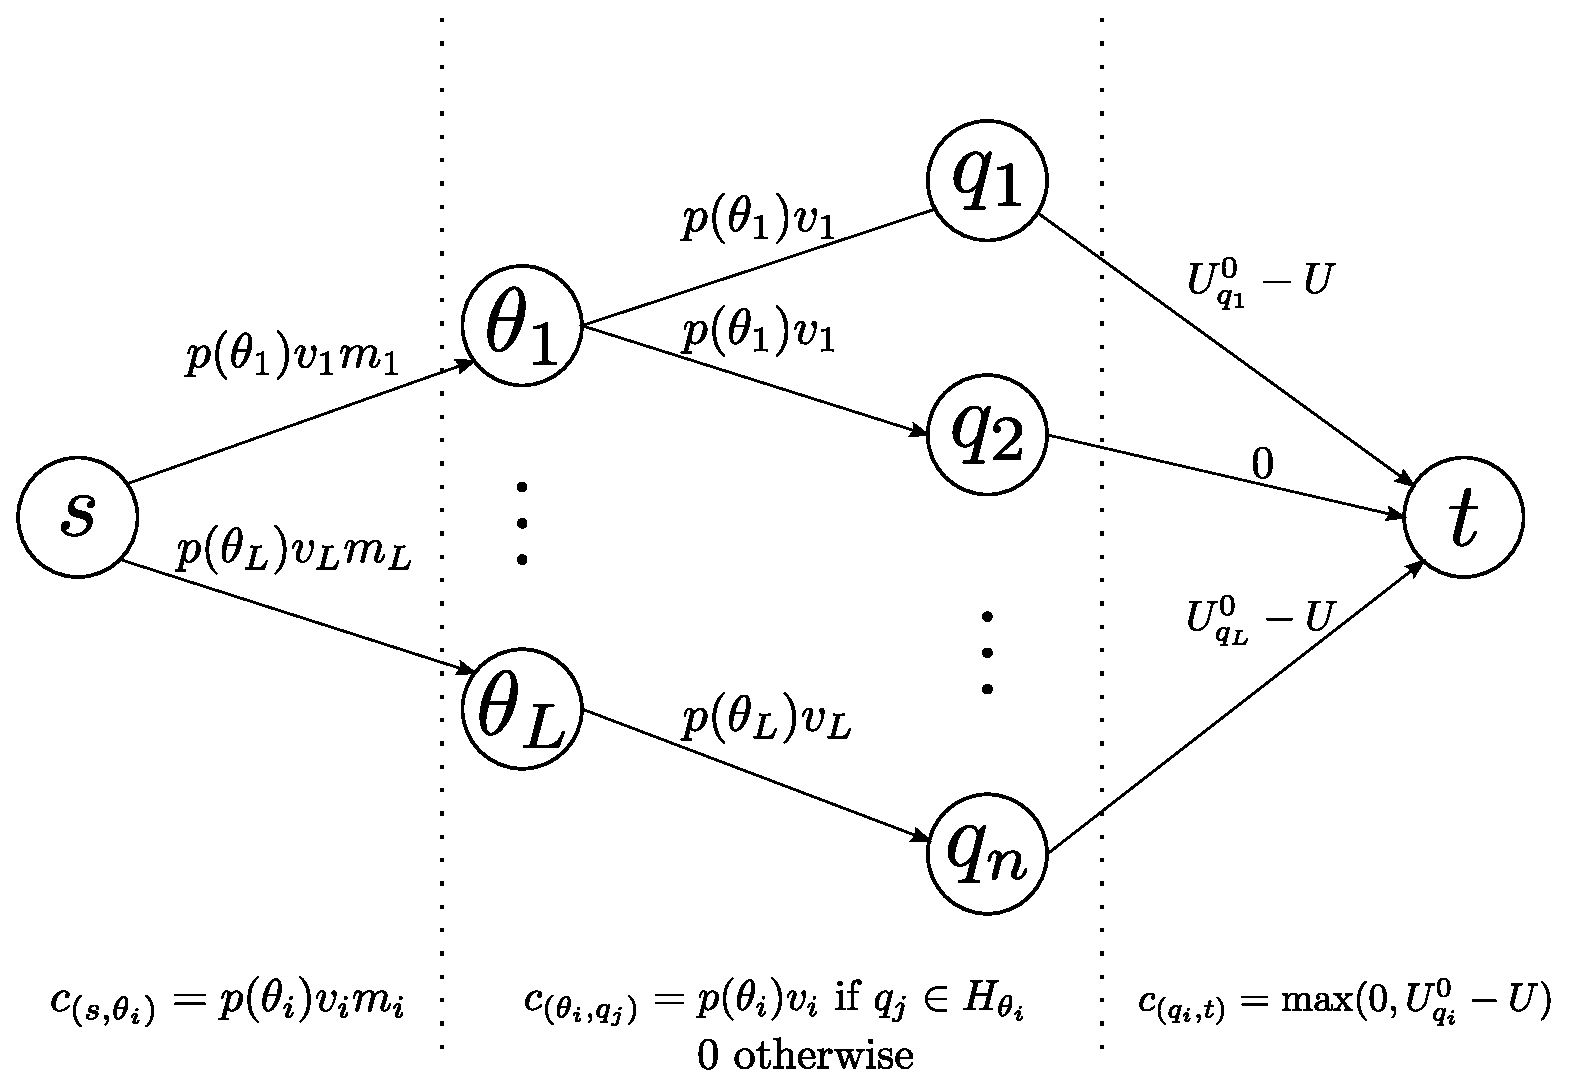
\includegraphics[trim=0 40mm 0 10mm, clip, width=\linewidth]{network}
\end{figure}

\begin{proposition}
The test network has a feasible flow that  saturates all the edges in $Q
\times \{t\}$ if and only if LP~(\ref{eqn:one-problem}) has a feasible
solution with value $U$.
\label{prop:network}
\end{proposition}
\begin{proof}
  If the test network has a feasible flow $f$ that saturates all the edges
  in $Q \times \{t\}$, then consider the solution to
  LP~(\ref{eqn:one-problem}) where $z_{\theta, q} = f_{(\theta, q)} /
  c_{(\theta, q)}$, so that clearly $0 \leq z_{\theta, q} \leq 1$.
 Because the $Q \times \{t\}$ edges are saturated, we
  have that for each $q \in Q$, $\sum_{\theta:q \in H_\theta}
  p(\theta)v_\theta z_{\theta,q} = \sum_{\theta:q \in H_\theta} f_{(\theta,
    q)} = \max(0, U_q^0-U) \geq U_q^0-U$, which implies $U \geq U_q^0 -
  \sum_{\theta:q \in H_\theta} p(\theta)v_\theta z_{\theta,q}$.  For each
  $\theta \in \Theta$, because of the capacity constraint on edge $(s,
  \theta)$, we have $\sum_{q \in H_\theta} z_{\theta,q} = (1/(p(\theta)
  v_\theta)) \sum_{q \in H_\theta} f_{(\theta, q)} \leq (1/(p(\theta)
  v_\theta)) f_{(s,\theta)} \leq (1/(p(\theta) v_\theta)) p(\theta) v_\theta
  m_\theta = m_\theta$.  Hence, we have a feasible solution to
  LP~(\ref{eqn:one-problem}) with objective value $U$.

  Conversely, if we have a feasible solution to LP~(\ref{eqn:one-problem})
  with objective value $U$, then set: (1) $f_{(\theta,q)} = 0$ if $U_q^0 \leq
  U$; (2) otherwise, set $f_{(\theta,q)} = \frac{U_q^0-U}{\sum_{\theta:q \in
      H_\theta} p(\theta)v_\theta z_{\theta,q}} z_{\theta,q} c_{(\theta,
    q)}$.  To satisfy the flow constraints, this implies $f_{(s,\theta)} =
  \sum_{q \in H_\theta} f_{(\theta,q)}$ and $f_{(q,t)} = \sum_{\theta: q \in
    H_\theta} f_{(\theta,q)}$.  We now check that the capacity constraints
  hold. By the first constraint in the LP, we have
  $\frac{U_q^0-U}{\sum_{\theta:q \in H_\theta} p(\theta)v_\theta z_{\theta,q}}
\leq 1$ so $f_{(\theta,q)}
    \leq z_{\theta,q} c_{(\theta, q)}$, and because $z_{\theta,q} \leq 1$
    we have that the capacity constraints on the  $\bigcup_{\theta \in \Theta} \{\theta\} \times
H_\theta$ edges
 are satisfied.  Then, we have $f_{(s,\theta)} = \sum_{q \in
      H_\theta} f_{(\theta,q)} \leq \sum_{q \in
      H_\theta} z_{\theta,q} c_{(\theta, q)} = 
p(\theta) v_\theta \sum_{q \in
      H_\theta} z_{\theta,q}  \leq p(\theta) v_\theta m_\theta =
    c_{(s,\theta)}$ by the second constraint of the LP. 
%vcDONE: check whether parentheses are in the subscripts of the capacities
  Finally, for any $q \in Q$, there are two cases: (1) if $U_q^0 \leq U$,
  then we have $f_{(q,t)} = \sum_{\theta: q \in H_\theta} f_{(\theta,q)} = 0$;
  (2) if $U_q^0 > U$, we have $f_{(q,t)} = \sum_{\theta: q \in H_\theta}
  f_{(\theta,q)} = \frac{U_q^0-U}{\sum_{\theta:q \in H_\theta}
    p(\theta)v_\theta z_{\theta,q}} \sum_{\theta: q \in H_\theta}
  z_{\theta,q} c_{(\theta, q)} = U_q^0-U$.  So the $Q \times \{t\}$ edges
  are exactly saturated.
\end{proof}

%If that network's max flow $f$ saturates all edges in $Q \times \{t\}$, then
%our $U$ is feasible and we found a solution $z_{\theta, q} = f_{(\theta, q)} /
%c_{(\theta, q)}$. 

We can do a binary search for the optimal value of $U$ to the desired level of
precision.\footnote{If an exact solution is desired, we can use a similar construction to
  reduce to the minimax network flow problem~\cite{Han199711}, where the goal is
  to compute a maximum flow that minimizes $\max_{e \in
    E'} f_e$ for some distinguished set of edges $E' \subseteq E$.  To do
  so, first (assuming w.l.o.g.~$U_{q_1}^0 \leq U_{q_2}^0 \leq U_{q_n}^0$)
  we use our algorithm above to find out in which interval $[U_{q_i}^0,
  U_{q_{i+1}}^0]$ the optimal $U$ lies.  Then, we modify the network by
  setting $c_{(q, t)} = \max(0, U_q^0-U_{q_{i+1}}^0)$ and find a flow that
  saturates these edges.  We consider the residual graph consisting of the
  remaining capacities, and again adjust the capacities $c_{(q, t)}$ from
  $0$ to $U_{q_{i+1}}^0-U_{q_i}^0$ whenever $U_q^0 \geq U_{q_i}^0$;
  finally, we can call a minimax network flow solver on this network with
  $E' = Q \times \{t\}$.  However, as we are not aware of any such
  solvers, in our experiments we focus on the approach based on binary search.}
%we can either do binary search for a
%finite precision, or use minimax network algorithm (see e.g.,
%\cite{}).\footnote{Our problem to minimize $U$ can be reduced to minimax
%network flow \cite{} which computes the max flow $f$ that minimizes $\max_{e
%\in E'} f_e$ in a predefined subset $E' \subseteq E$, by: firstly use binary
%search to find out the interval $[U_{q_i}^0, U_{q_{i+1}}^0]$ that includes our
%minimum $U$ (W.l.o.g, assuming that $U_{q_1} \leq U_{q_2} \leq \ldots$); then
%find a max flow by setting $c_{(q, t)} = \max(0, U_q^0-U_{q_{i+1}}^0)$ (and we
%shall saturate them); in the residual graph, reset residual capacity $c_{(q,
%t)}$ from $0$ to $U_{q_{i+1}}^0-U_{q_i}^0$ if $U_q^0 \geq U_{q_i}^0$; finally
%find out the max flow that minimizes $\max_q f_{(q, t)}$.} 
The proof of Proposition~\ref{prop:network} shows us how to find the 
 test taker's strategy corresponding to a particular flow.


\subsection{A Direct Algorithm for Identifying the Tester's Strategy}

We now give a direct algorithm (Algorithm~\ref{alg:one-problem}) that, given an equilibrium strategy for the
test taker, computes an equilibrium strategy for the tester.
%The network flow only computes the strategy for test takers. Since we are more
%interested in tester's strategy, we construct them by the following
%Algorithm~\ref{alg:one-problem}.
This also allows us to prove that there always exists such a strategy where
the tester uniformly randomizes over a subset of the questions (rather
than, for example, placing high probability on a question that is hard for
many types and low, but nonzero, probability on a question that is hard for
fewer types).


%We can also explicitly construct the tester's optimal strategy from the dual
%solution using Algorithm~\ref{alg:one-problem}, which always return a strategy
%that tests a subset of questions uniformly.

\begin{algorithm}
\caption{Input: A test game with $t = 1$ and an optimal primal solution $(U, (z_{\theta,q}))$ to LP~(\ref{eqn:one-problem}).}
%Compute the optimal test strategy with size one, given the optimal
%utility $U$ and test takers strategy $z$, which is either computed by
%LP~(\ref{eqn:one-problem}) or the network flow algorithm we described
%above.}
\label{alg:one-problem}
\begin{algorithmic}[1]
%\Function{OptimalOneProblemTest}{$Q, \Theta, p, U, z$}
%	\State Solve LP~(\ref{eqn:one-problem}) and let the solution be $U,
%	z_{\theta,q}$
	\State $T \gets \{q ~|~ U^0_q  - \sum_{\theta: q \in H_\theta}
        p(\theta) v_\theta z_{\theta,q} = U\}$
	\State $S \gets \{\theta : \sum_{q \in H_\theta \cap T} z_{\theta,q} < m_\theta\}$
	%\ForAll {$B_l \in Q$} \Comment{Potential Memorizing Power}
	%	\State $G(B_l) \gets m_l-\sum_{a \in B_l \cap T} z_{l,a}$ 
	\label{line:first-potential}
	%\EndFor
	\While{$S$ has an unmarked element}
		\State $\theta \gets $ an unmarked element from $S$
		\ForAll{$q \in H_\theta \cap T$ and $z_{\theta,q} < 1$}
			\State $S \gets S \cup \{\theta' \in \Theta: q \in
                        H_{\theta'} \wedge z_{\theta', q}>0\}$
			\State $T \gets T \setminus \{q\}$\label{line:delete-a}

			%\ForAll {$\theta': q \in H_\theta$ and $z_{\theta', q}>0$}
				%\State $G(B_{l'}) \gets \min(z_{l',a}, \frac{G(B_l)}{|B_l|L})$
				\label{line:second-potential}
		%	\State Push $\theta'$ into $Q$
			\label{line:second-push}
		%	\EndFor
		\EndFor
	\State mark $\theta$
	\EndWhile
	\State \Return{the uniform distribution over $T$}
%\EndFunction
\end{algorithmic}
\end{algorithm}

\begin{figure*}
\centering
	\subfigure[Increasing $n$ with \newline $L = 150$ and $m_{\text{max}} = 6$.]{
		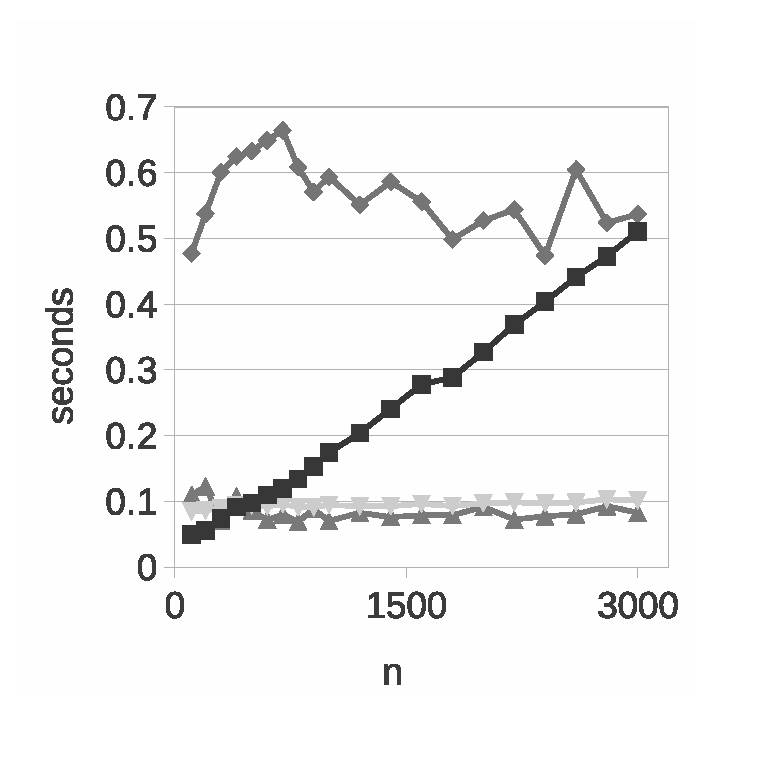
\includegraphics[trim=0 10mm 15mm 10mm, clip, height=1.3in]{small_n}
		\label{fig:individual_n}
	}
	\subfigure[Increasing $L$ with \newline $n = 150$ and $m_{\text{max}} = 6$.]{
		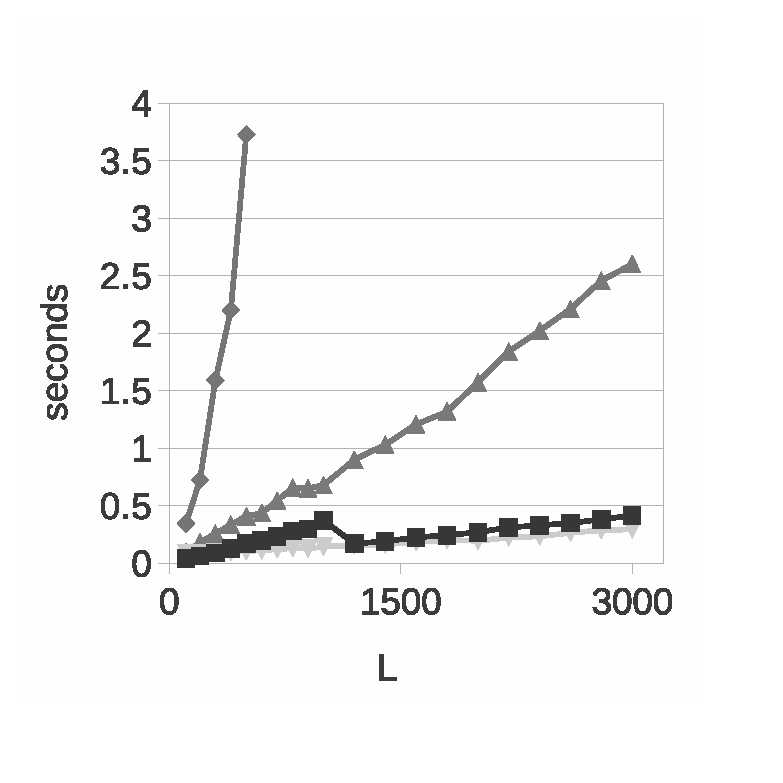
\includegraphics[trim=0 10mm 15mm 10mm, clip, height=1.3in]{small_L}
		\label{fig:individual_L}
	}
	\subfigure[Increasing $m_\text{max}$ with \newline $n = L = 150$.]{
		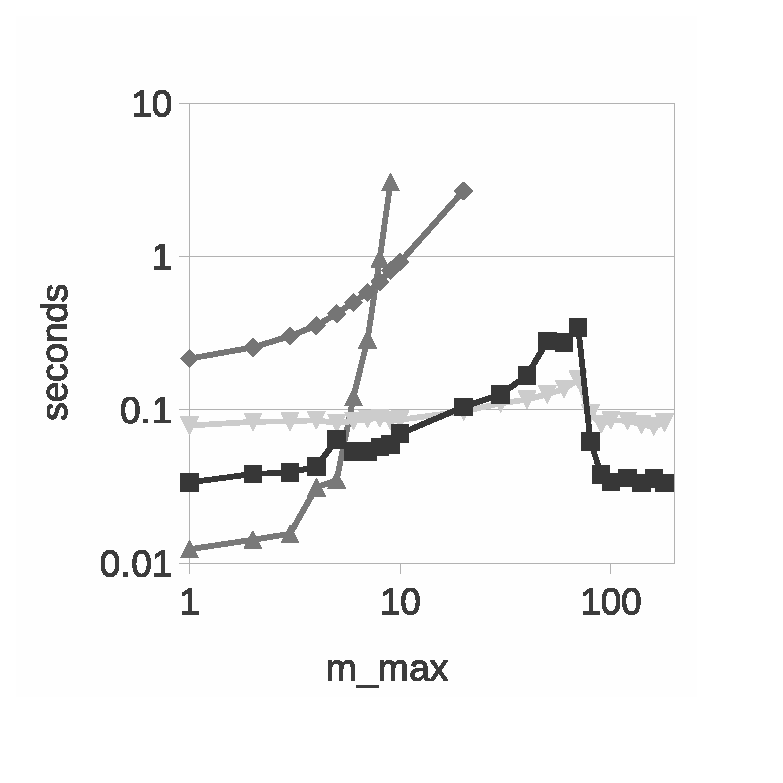
\includegraphics[trim=0 10mm 15mm 10mm, clip, height=1.3in]{small_m}
		\label{fig:individual_m}
	}
	\subfigure[Increasing $n$ with $L = n$ \newline and
			$m_{\text{max}} = \lfloor \sqrt{n} \rfloor$.]{
		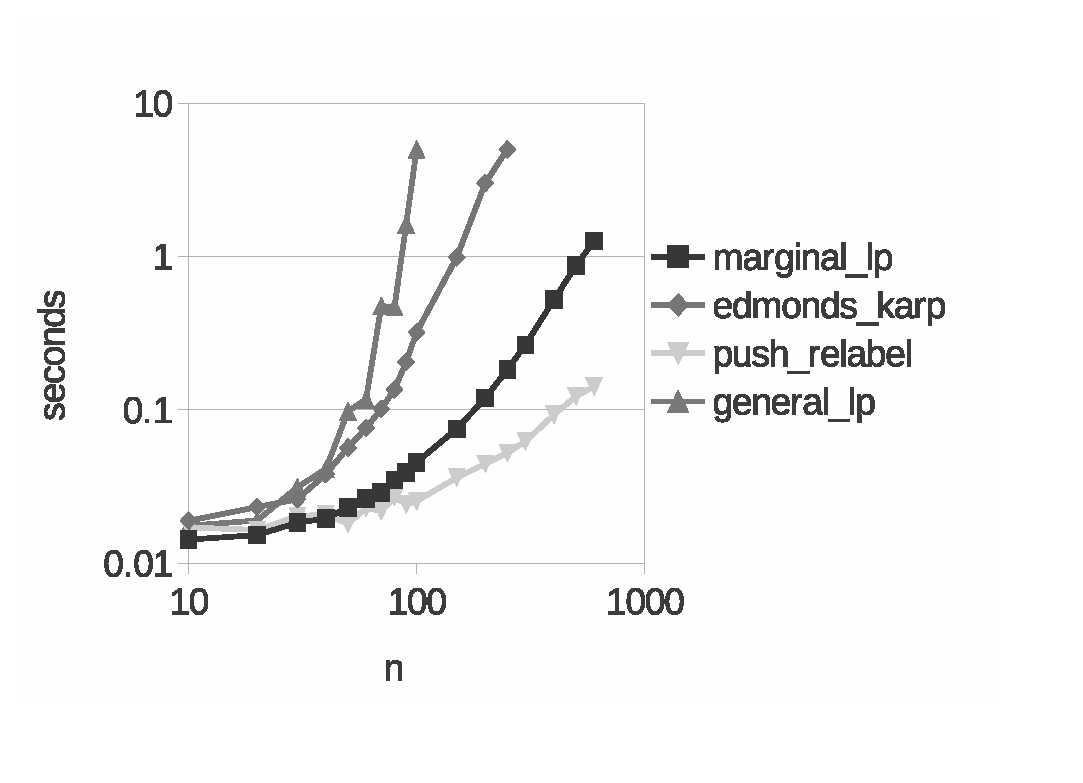
\includegraphics[trim=0 10mm 20mm 10mm, clip, height=1.3in]{small_combined}
		\label{fig:benchmark}
	}
	\caption{Runtime for solving for an optimal tester strategy in one-question tests.}
\end{figure*}

To  prove the correctness of Algorithm~\ref{alg:one-problem}, we first
introduce the following two lemmas.

\begin{lemma}\label{lemma:non-empty}
At every point in Algorithm~\ref{alg:one-problem}, $T$ is nonempty.
\end{lemma}

\begin{proof}
$T$ is non-empty initially, because otherwise $U$ would clearly be suboptimal.
%before we delete problems from $T$ on line~\ref{line:delete-a}
%of Algorithm~\ref{alg:one-problem}.  
Let $T_0$ denote that initial $T$.  Suppose that at some point, all
questions in $T_0$ are deleted.  We will show how to construct an
alternative solution $(z'_{\theta,q})$ such that for each $q \in T_0$, we
have 
$\sum_{\theta \in
  \Theta: q \in H_\theta}p(\theta)v_\theta z'_{\theta,q} > \sum_{\theta \in
  \Theta: q \in H_\theta}p(\theta)v_\theta z_{\theta,q}$.  This would then allow us
  to reduce $U$, contradicting its optimality.

  We initialize $z'_{\theta,q} = z_{\theta, q}$ for all $\theta, q \in T_0
  \cap H_\theta$, and $z'_{\theta,q} = 0$ otherwise.  Then, we will adjust
  the $z'_{\theta, q}$ for $q \in T_0$ in the same order in which these $q$
  were eliminated from $T$.  We maintain the property that, if $q$ is the
  latest question for which we have adjusted the $z'_{\theta,q}$, then for
  all $\theta \in S_q$ (where $S_q$ is the subset $S$ in the algorithm
  after eliminating $q$), we have $\sum_{q \in H_\theta} z'_{\theta,q} <
  m_\theta$.  This property holds initially by the initialization of $S$.
  When we reach $q \in T_0$, because it was eliminated, there is a $\theta
  \in S$ such that $z'_{\theta,q} < 1$. Let $\epsilon = (1 - z'_{\theta,q})/2$.
Then, let $z'_{\theta,q} \leftarrow z'_{\theta,q} + \epsilon$ and, for
every $\theta' \in \Theta$ such that $q \in H_{\theta'}$ and $z'_{\theta',q}
>0$, let  $z'_{\theta',q} \leftarrow  z'_{\theta',q} - \min(z'_{\theta',q},
\frac{\epsilon}{2 |\Theta|} \frac{p(\theta)v_\theta}{p(\theta')v_{\theta'}})$,
thereby maintaining the property. 
As a result, $\sum_{\theta'' \in
  \Theta: q \in H_{\theta''}}p(\theta'')v_{\theta''} z'_{\theta'',q}$ will have
increased by at least  $\epsilon p(\theta)v_{\theta} - \sum_{\theta' \in
\Theta} p(\theta')v_{\theta'} \frac{\epsilon}{2 |\Theta|}
\frac{p(\theta)v_\theta}{p(\theta')v_{\theta'}}  = 
\epsilon p(\theta)v_{\theta} - |\Theta| \frac{\epsilon}{2 |\Theta|} p(\theta)v_\theta >0$.
Hence, at the end, for each $q \in T_0$, we
have 
$\sum_{\theta \in
  \Theta: q \in H_\theta}p(\theta)v_\theta z'_{\theta,q} > \sum_{\theta \in
  \Theta: q \in H_\theta}p(\theta)v_\theta z_{\theta,q}$.
%vcDONE: be consistent about L vs |\Theta|
%Note that for every $\theta$ in $S$, it
%has a potential to memorize more either because $\sum_{q \in H_\theta \cap T_0}
%z_{l,a} < m_l$ (on line \ref{line:first-potential}) or because there is an
%unnecessary memorizing $z_{\theta, q} > 0$ that can be freed (on line
%\ref{line:second-potential}). So all questions in $T_0$ being deleted means
%that we can bring $U$ down by using those potentials to memorize all questions
%in $T_0$ more (recall $\forall q \in T_0, \exists \theta, z_{\theta,q} <
%1$), a contradiction to that $U$ is minimized.  
\end{proof}

\begin{lemma}\label{lemma:best-response}
Let $(z_{\theta,q})$ be the solution to LP~(\ref{eqn:one-problem}) and let $T$ be the
final subset that Algorithm~\ref{alg:one-problem} returns. Then for each type
$\theta$, either $\sum_{q \in H_\theta \cap T} z_{\theta,q} = m_\theta$
($\theta$ memorizes as much of  $T\cap H_\theta$ as possible) or $\forall q \in
H_\theta \cap T, z_{\theta, q} = 1$ ($\theta$ memorizes every question in $T\cap
H_\theta$ with probability $1$ and will certainly pass the test). Therefore
all types of test taker are best-responding.
\end{lemma}

\begin{proof}
  We will show that the algorithm maintains the following properties after
  initialization of $T$ and $S$.  (1) Any type $\theta \in \Theta$ for
  which $\sum_{q \in H_\theta \cap T} z_{\theta,q} < m_\theta$ is in $S$.
  (2) All marked types $\theta$ satisfy $\forall q \in H_\theta \cap T,
  z_{\theta, q} = 1$.  From this, the lemma follows, because at the end of
  the algorithm, the condition for the {\bf while} loop must be false, so
  every type must be either not in $S$, in which case the first condition
  in the lemma holds, or marked, in which case the second condition holds.

  Clearly (1) and (2) hold after initialization.  For any $\theta$, the
  only way in which $\sum_{q \in H_\theta \cap T} z_{\theta,q}$ can
  decrease is if some $q \in H_\theta$ with $z_{\theta,q} > 0$ is removed
  from $T$; but in that case, in the preceding line of the algorithm,
  $\theta$ will have been added to $S$.  This proves (1) is maintained.
  When some $\theta$ is marked, all $q \in H_\theta$ such that
  $z_{\theta,q} < 1$ have just been removed from $T$. This proves (2)
 is maintained.
%Let $T_0$ be the initial $T$ before any deletion on line~\ref{line:delete-a} of
%Algorithm~\ref{alg:one-problem}.  Initially, for any $\theta$ such that
%$\sum_{q \in H_\theta cap T_0} z_{\theta,q} < m_\theta$, we push it to $S$.
%After that any $q \in H_\theta$ where $z_{\theta,q} < 1$ is deleted from $T$ on
%line~\ref{line:delete-a}.  Therefore $\forall q \in H_\theta \cap T,
%z_{\theta,q} = 1$ must hold for that $\theta$.  Afterwards, more $\theta$ may
%violate $\sum_{q \in H_\theta cap T} z_{l,a} = m_l$ because some $q$ are
%deleted from $T$.  But for those $H_\theta$, we must have pushed them into $S$
%on line~\ref{line:second-push}. So they will satisfy $\forall q \in H_\theta
%\cap T, z_{\theta,q} = 1$ afterwards. In the end, every $\theta \in S$ will
%satisfy $\forall q \in H_\theta \cap T, z_{\theta,q} = 1$ and every other
%$\theta \notin Q$ will satisfy $\sum_{q \in H_\theta \cap T} z_{\theta,q} =
%m_l$.
\end{proof}

%Then we show our strategy is optimal by complementary slackness theorem, which
%in our context is essentially: 1) the tester only tests problems (non-zero
%primal variables) that gives him best utility (tight dual constraints); 2) the
%test taker only memorizes problems (non-zero dual variables) that gives him
%best utility (tight primal constraints).\footnote{This is essentially saying
%that in a zero-sum game, a minimax, or maximin state is reached, if and only if
%the Nash equilibrium is reached.} 

\begin{theorem}
Let $(z_{\theta,q})$ be the solution to LP~(\ref{eqn:one-problem}) and
$(x_q)$ the uniform distribution over the set 
 $T$ returned by Algorithm~\ref{alg:one-problem}.  Then
 $((x_q),(z_{\theta,q}))$ constitute an equilibrium.\footnote{By
   complementary slackness, this also means they constitute optimal primal
   and dual solutions to our LPs.}
\end{theorem}
\begin{proof}
By Lemma~\ref{lemma:non-empty}, $(x_q)$ is a valid strategy. 
%First of all, $T$ is non-empty by Lemma~\ref{lemma:non-empty} so we can test
%$T$ uniformly. 
By the initialization of $T$, $T$ can ever only include questions
that give the tester the maximum utility $U$.
%Then since memorizing strategy $z_{\theta,q}$ makes $U_q$ (the
%utility to test a problem $q$) decrease to $U$ if $U^0_q > U$ and we only pick
%$T$ from problems that $U^0_q > U$, every problem that we might test gives the
%tester best utility. That is the first condition for the complementary
%slackness theorem.  
Finally, Lemma~\ref{lemma:best-response} shows that all test taker types
are best-responding.
%one
%type of test takers either pass the test for sure or memorize the maximal
%subset in $H_\theta \cap T$ all the time which is optimal for uniform test, the
%second condition of complementary slackness theorem holds.
\end{proof}


%Finally, instead of using general LP algorithm like simplex [cite] to solve
%LP~(\ref{eqn:one-problem}), we can alternatively use binary search plus max
%flow to solve it as shown in Algorithm~\ref{alg:max-flow}.  With a given $U$,
%we use max flow to check its feasibility. Intuitively, a $U$ is feasible if and
%only if there is a strategy $z_{l, a}$ such that for every $a$ where $U^0_a >
%U$, that strategy decreases it down to $U$. This is achievable if and only if
%the max flow can saturate all edges from $A$ to $t$. Given a max flow $f$, we
%can restore the strategy by setting $z_{l, a} = f_{(B_l, a)}/c_{(B_l, a)}$
%which is the flow of an edge divded by the capacity of an edge. If we use
%Push-Relabel algorithm [cite] to solve the max flow in $O((n+L)^3)$ time, the
%whole Algorithm~\ref{alg:one-problem} runs in $O((n+L)^3 + \sum_l |B_l|)$ time
%as the remaining part can run in linear time with repsect to the input size
%(assuming we only binary search for constant times to achieve a constant
%accuracy).
%
%\begin{algorithm}
%\caption{Use binary search and max flow to solve LP~(\ref{eqn:one-problem})}
%\label{alg:max-flow}
%\begin{algorithmic}[1]
%	\State $U_{lower} \gets 0, ~U_{upper} \gets \max_{a \in A} U^0_a$
%	\While{$U_{upper}-U_{lower} > \epsilon$}\Comment{Binary search}
%		\State $U \gets (U_{upper}+U_{lower})/2$ \Comment{Objective utility}
%		\State $V \gets \{s\} \cup \mathbb B \cup A \cup \{t\}$ \Comment{Vertex set}
%		\State $E \gets \emptyset$ \Comment{Initialize edge set}
%		\ForAll{$a \in A$}
%			\If{$U^0_a > U$}
%				\State $E \gets E \cup \{(a, t)\}$
%				\State $c_{(a, t)} \gets U^0_a-U$ \Comment{Edge capacity}
%			\EndIf
%		\EndFor
%		\ForAll{$B_l \in \mathbb B$} 
%			\State $E \gets E \cup \{B_l\} \times B_l$ %\Comment{Edges between $\mathbb B$ and $A$}
%			\State $c_{\{B_l\} \times B_l} \gets p_l v_l$ 
%			\State $E \gets E \cup \{(s, B_l)\}$ %\Comment{Edges between $\{s\}$ and $\mathbb B$}
%			\State $c_{(s, B_l)} \gets p_l m_l v_l$
%		\EndFor
%		\State $f \gets \Call{MaxFlow}{G = (V, E), c}$
%		\If{$f$ saturates all edges in $A \times \{t\}$}
%			\State $U_{upper} \gets U$
%		\Else
%			\State $U_{lower} \gets U$
%		\EndIf
%	\EndWhile
%	\State $(\forall l, a), z_{l,a} \gets f_{(B_l,a)} / c_{(B_l, a)}$
%	\State \Return{$U, z_{l,a}$}
%\end{algorithmic}
%\end{algorithm}

\section{Experiments}

In this section, we describe experiments that we performed to see how
different algorithms scale. We also show how the optimal test strategy
outperforms simple test strategies, such as drawing questions uniformly at
random.
% (e.g. draw a test uniform at random) in
%terms of tester's utility.

\subsection{Tests of Size 1: Scalability}

We first restrict our attention to single-question test games, in which we
can evaluate all our algorithms at once.
%while LP~(\ref{eqn:maximin}) (and its dual LP~{\ref{eqn:dual-original})
%also work for tests with more questions, as we will see, one-question test
%games are already challenging for these formulations.
We consider four different algorithms.  We use CPLEX (out-of-the-box)
to solve (1) the general LP~(\ref{eqn:maximin}) and (2) the one-question
marginal-probabilities LP~(\ref{eqn:one-problem}).  Also, we use the
network-flow approach from Definition~\ref{def:network} with binary search
on $U$ to a precision of $10^{-8}$ using (3) Edmonds-Karp \cite{Edmonds:1972} and (4)
Push-Relabel \cite{Goldberg:1988:NAM:48014.61051}, in each case combined with 
Algorithm~\ref{alg:one-problem} to compute the tester's optimal strategy.
% The first approach is using CPLEX to solve our
%general LP~(\ref{eqn:maximin}) which is exponential to the memorize capacity.
%The second one is using CPLEX to directly solve the marginal version
%LP~(\ref{eqn:one-problem}). The third and fourth use Edmonds-Karp [cite] and
%Push-Relabel [cite] max flow algorithm respectively (with binary search) on the
%network defined in Definition~\ref{def:network} and then use
%Algorithm~\ref{alg:one-problem} to compute the tester's optimal strategy.

In particular, we use CPLEX 10.010 and the boost 1.46.1 C++ library
for Edmonds-Karp and Push-Relabel.
%\footnote{We increased the tolerance 
%on its is\_flow function
%to address floating number issues.} 
%max flow implementation. 
Our machine has an
Intel i7-2600 3.40GHz CPU and 8GB memory.
%flow algorithm respectively
%to solve LP~(\ref{eqn:one-problem} and then use
%????Algorithm~\ref{alg:max-flow} to solve LP~(\ref{eqn:one-problem}). They are
%using Edmonds-Karp [cite] and Psh-Relabel [cite] max flow algorithm in C++ boost
%library respectively.

%Therefore
%we focused on comparing different varieties of
%Algorithm~\ref{alg:one-problem}. In high level, there are two different
%ways to implement: one is solving LP~(\ref{eqn:one-problem}) using general LP
%algorithm and the other is solving it using max flow as shown in
%Algorithm~\ref{alg:max-flow}. In low level, we compared glpk and cplex for
%general LP solving methods and compared Edmonds-Karp [cite] and
%Push-Relabel\footnote{We modified its is\_flow function for floating number
%issues.} [cite] using C++ boost library [cite] for max flow methods.  In
%summary, we have four varieties in our comparisons.

For each experimental data point, we specify three parameters:
the number of questions $n$, the number of types $L$ ($|\Theta| = L$), and the maximum
memory size $m_{\text{max}}$.  We always set $b_\text{max}$, the maximum
size of any $H_\theta$, to $2m_{\text{max}}$.
% $n, L,
%m_{max}, b_{max}$, the number of problems, the number of test taker types,
%the maximum memorize capacity and the maximum size of $B_l$. 
Given those
parameters, a test game instance is randomly generated as follows: for each
$\theta \in \Theta$, draw $m_\theta$ uniformly from $1$ to $m_{\text{max}}$; draw $|H_\theta|$
uniformly from $m_\theta$ to $b_{\text{max}}$;
generate $H_\theta$ by drawing $|H_\theta|$
elements from $Q$ uniformly; and draw $w_\theta = p(\theta)v_\theta$ 
uniformly 
from $[0,1]$ (these two factors always appear together).
%. Here we only generate $w_l$ because $v_l$
%and $p_l$ always appear together as $v_l p_l$. 
For each data point,
we generate $5$ test game instances and compute the average running time
for each algorithm.  We set a timeout of 5 seconds for each instance.


%\subsection{Test with Individual Parameter}


Figures~\ref{fig:individual_n},~ \ref{fig:individual_L},
and~\ref{fig:individual_m}  show how the algorithms scale in $n$, $L$, and
$m_\text{max}$, respectively, holding the other parameters fixed.  
(Note the logarithmic scales on Figure~\ref{fig:individual_m}.)
None of the algorithms have trouble scaling in $n$ alone.
 Edmonds-Karp does not scale very well in $L$ and
$m_\text{max}$, and the general LP scales particularly poorly in
$m_\text{max}$.
The marginal LP and particularly push-relabel always scale very well.
%, and
%they also show that once $m_\text{max}$ reaches a particular size, thes
%In this benchmark, we fix the other three parameters and change the other one. The results are
%shown in Figure~\ref{fig:individual_n}, \ref{fig:individual_L}, \ref{fig:individual_m}.

%\begin{figure}
%	\caption{Runtime for increasing $n$
%with 
%$L = 150$ and $m_{\text{max}} = 6$.}\label{fig:individual_n}
%	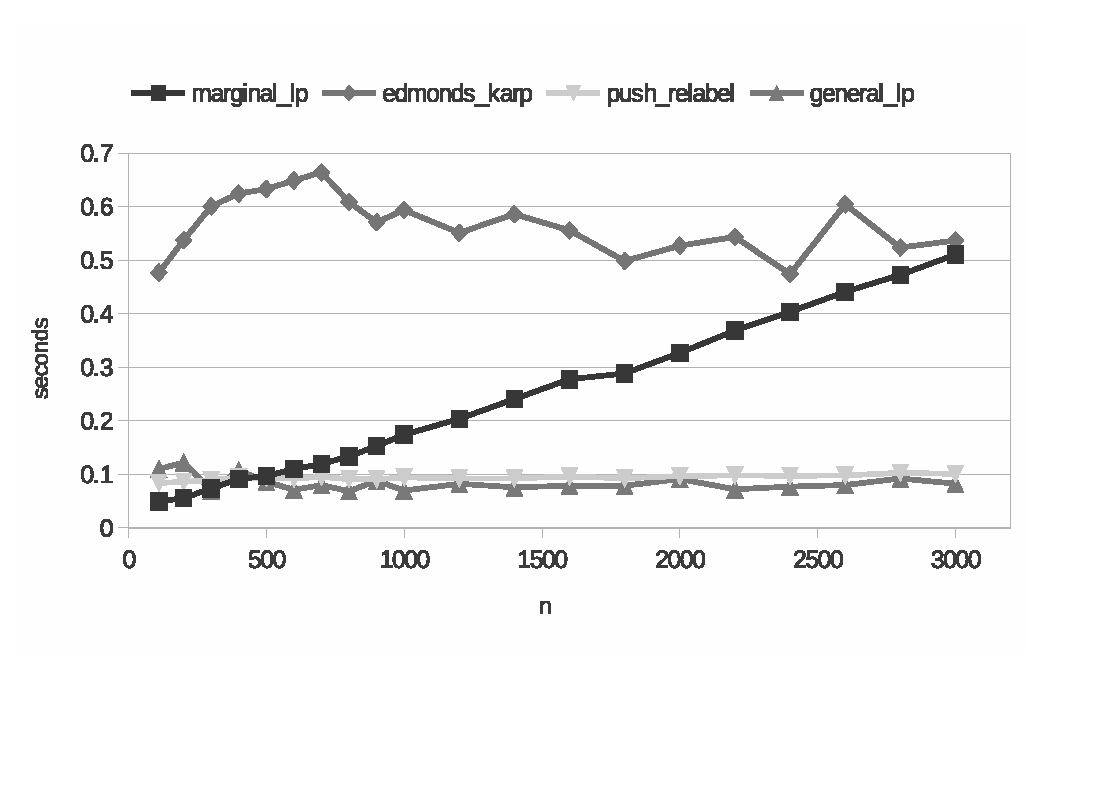
\includegraphics[trim=0 20mm 0 0, clip, width=\linewidth]{individual_n}
%\end{figure}
%
%\begin{figure}
%	\caption{Runtime for increasing $L$ with 
%$n = 150$ and $m_{\text{max}} = 6$.}\label{fig:individual_L}
%	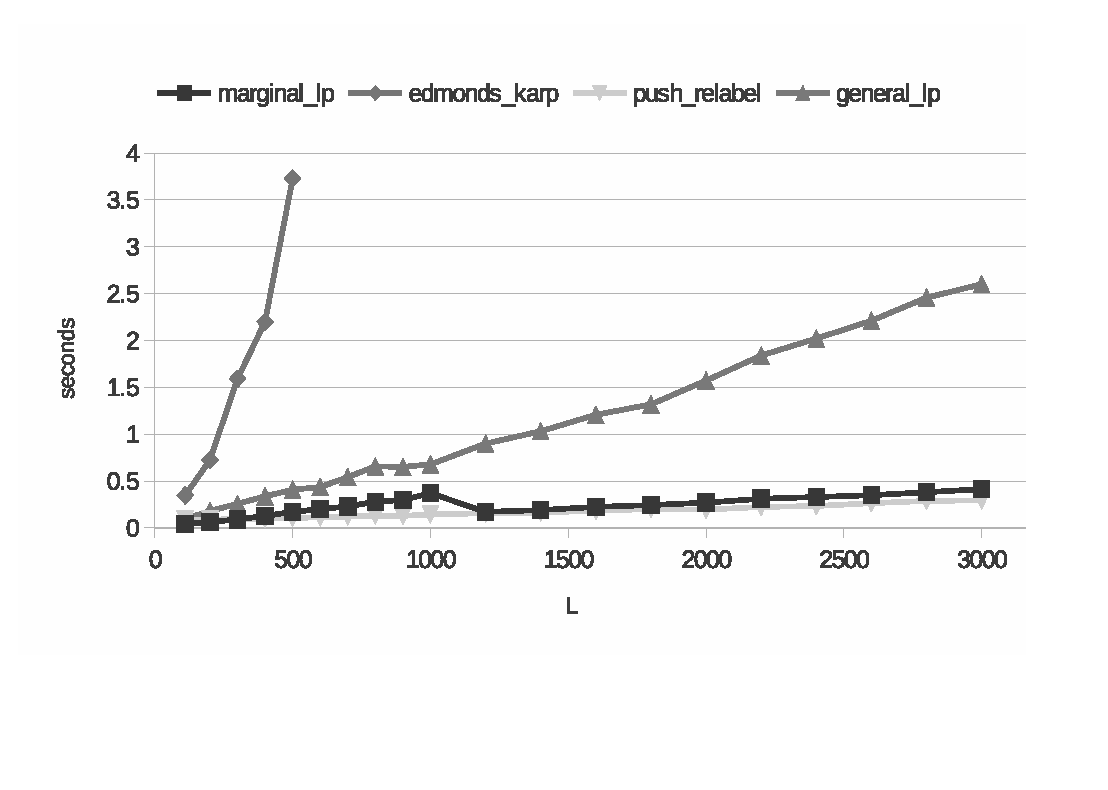
\includegraphics[trim=0 20mm 0 0, clip, width=\linewidth]{individual_L}
%\end{figure}
%
%\begin{figure}
%	\caption{Runtime for increasing $m_{max}$ with 
%$n = 150$ and $L = 150$.}\label{fig:individual_m}
%	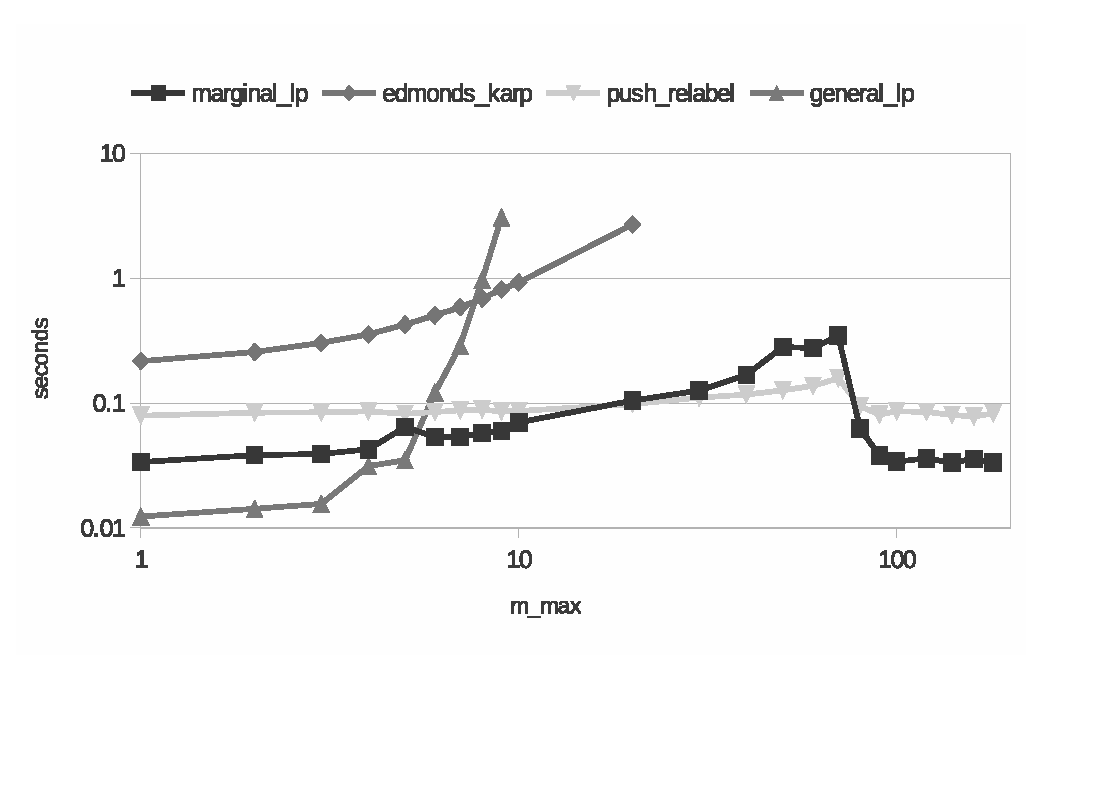
\includegraphics[trim=0 20mm 0 0, clip, width=\linewidth]{individual_m}
%\end{figure}
%vcDONE: put captions below figures


In fact, these experiments indicate increasing a single parameter by itself
never leads to truly hard instances.  For $n$ eventually many of the
questions become irrelevant (not hard for any type).  For $L$ and
$m_\text{max}$, eventually it becomes optimal to randomize uniformly over
all questions.
Thus, to identify more challenging instances, multiple parameters need to
increase simultaneously, as we do in Figure~\ref{fig:benchmark} (note again
the logarithmic scales).  Push-relabel performs best.



%\subsection{Test with Correlated Parameters}

%\begin{figure}
%	\caption{Runtime for increasing $n$ with  $L = n$ and 
%	$m_{\text{max}} = \lfloor \sqrt{n} \rfloor$.}
%	\label{fig:benchmark}
%	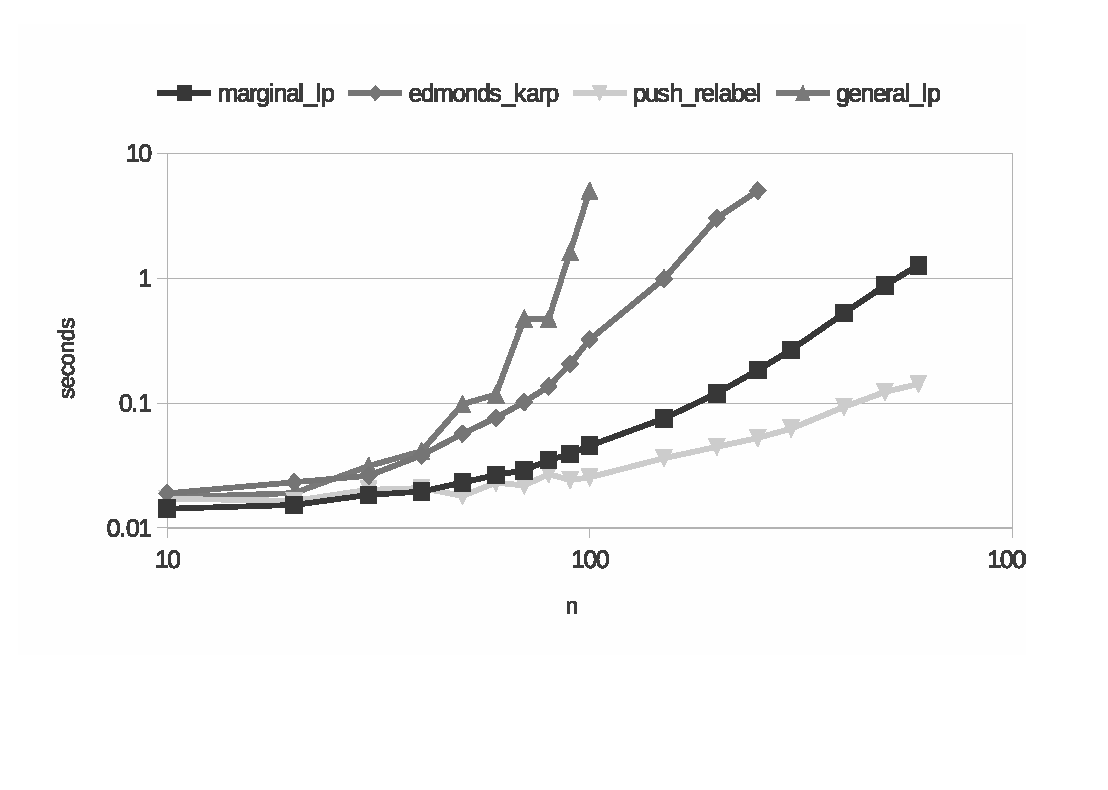
\includegraphics[trim=0 20mm 0 0, clip, width=\linewidth]{combined}
%\end{figure}

%In this benchmark, we increase $n$ and set the remaining three parameters $L,
%m_{max}, b_{max}$ as following: $L = n, m_{max} = \lfloor \sqrt{n} \rfloor$ and
%$b_{max} = 2m_{max}$. Note that our $L, b_{max}$ are quite small (they can be
%as large as $b_{max} = n/2, L = \binom{n}{b_{max}})$. That's becuase for large
%$L, b_{max}$, our uniform random input will almost always make the trivial
%strategy to uniformly test among all $n$ problems optimal. So we make them
%small to avoid such trivial solutions. The realized parameter settings are
%shown in Table~\ref{tab:settings}. The benchmark is shown in
%Figure~\ref{fig:benchmark}.  As expected, the general LP is exponential so it
%times out before $n$ reaches $100$.  Unexpectedly, using CPLEX to directly
%solve LP~(\ref{eqn:one-problem}) is much faster than Edmonds-Karp
%implementation. Finally, Push-Relabel version outperforms all others
%significantly. It solves $n=1000$ case in about $0.5$ second while the second
%best CPLEX version uses almost 5 seconds.

%\begin{table}
%	\caption{Parameter settings for the benchmark}\label{tab:settings}
%	\begin{center}
%	\begin{tabular}{ r r r r }
%		$n$&$L$&$m_{max}$&$b_{max}$\\
%		\hline\\
%		10&	10&	3&	6 \\ 
%		20&	20&	4&	8 \\
%		30&	30&	5&	10\\
%		40&	40&	6&	12\\
%		50&	50&	7&	14\\
%		60&	60&	7&	14\\
%		70&	70&	8&	16\\
%		80&	80&	8&	16\\
%		90&	90&	9&	18\\
%		100&100&10&20\\
%		150&150&12&24\\
%		200&200&14&28\\ 
%		250&250&15&30\\
%		300&300&17&34\\
%		350&350&18&36\\
%		400&400&20&40\\
%		450&450&21&42\\
%		500&500&22&44\\
%		550&550&23&46\\
%		600&600&24&48\\
%		650&650&25&50\\
%		700&700&26&52\\
%		750&750&27&54\\
%		800&800&28&56\\
%		850&850&29&58\\
%		900&900&30&60\\
%		950&950&30&60\\
%		1000&1000&31&62
%	\end{tabular}
%	\end{center}
%\end{table}

\subsection{Tests with Multiple Questions: Scalability}

When the test can contain more than one question, the only algorithm that
we have provided is our general LP~(\ref{eqn:maximin}).  We compare this with the standard
solver for Bayesian Stackelberg games, DOBSS~\cite{Paruchuri08:Playing}
(using the same version of CPLEX).
%We consider two algorithms, one is the DOBSS MIP for general Bayesian
%Stackelberg games and the other is our minimax LP which exploits the zero-sum
%modification of our test games. 
The machine we use and the way we generate test
game instances (other than the number of questions) remain the same as in the previous subsection.

\begin{figure*}
	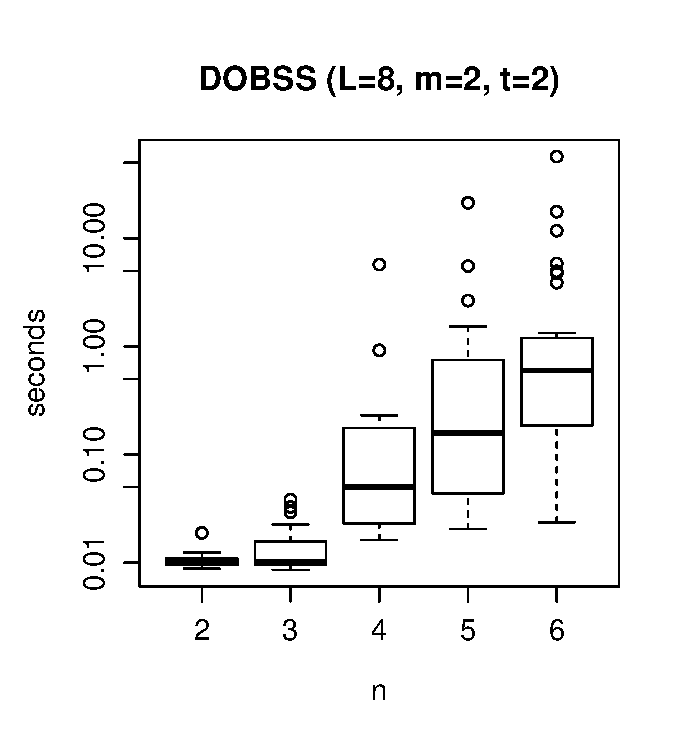
\includegraphics[width=.23\linewidth]{multi/DOBSS_n}
	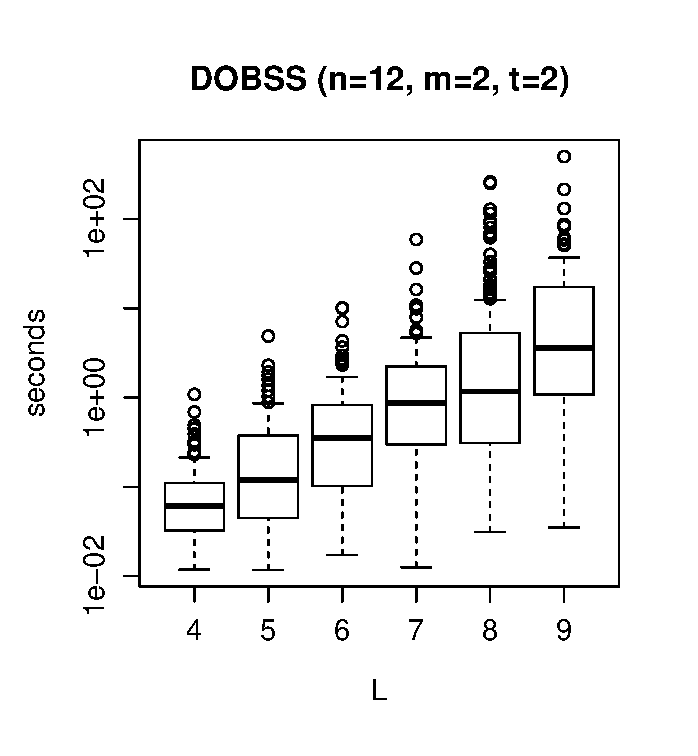
\includegraphics[width=.23\linewidth]{multi/DOBSS_L}
	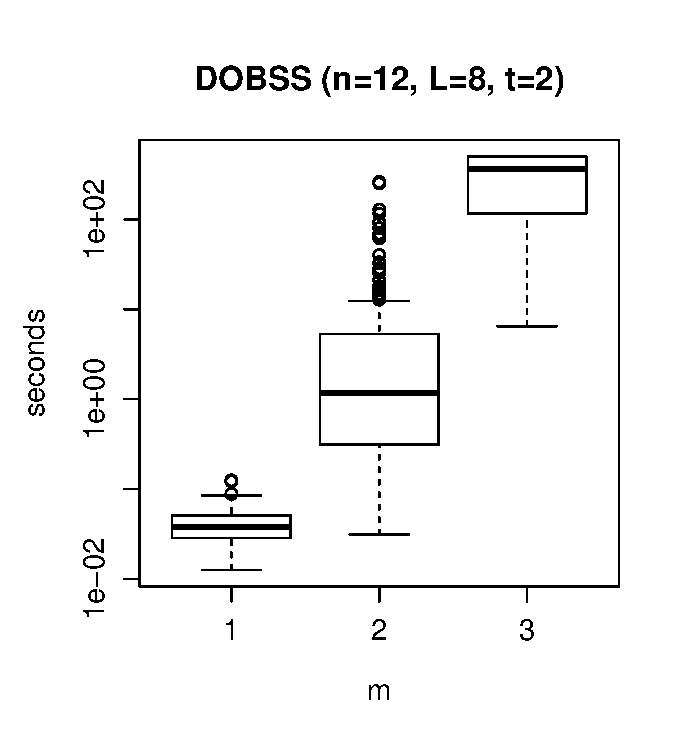
\includegraphics[width=.23\linewidth]{multi/DOBSS_m}
	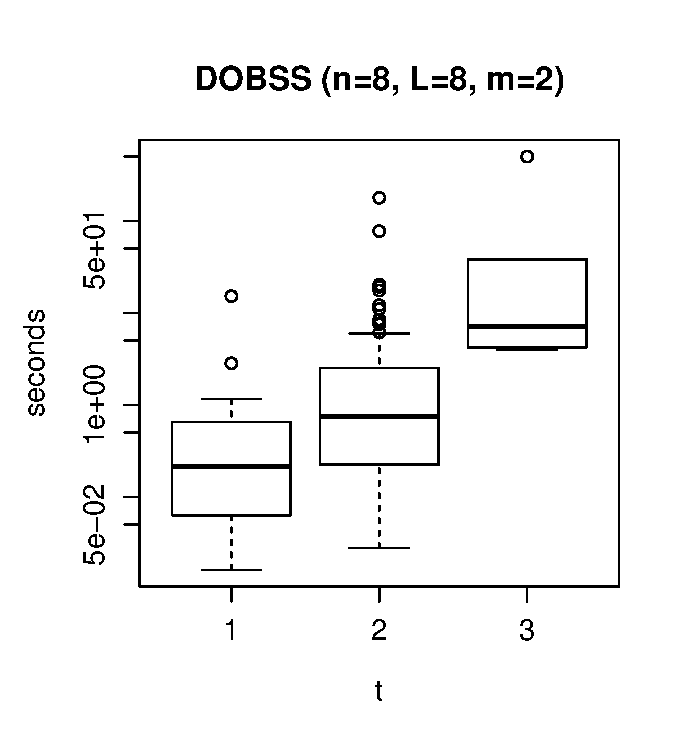
\includegraphics[width=.23\linewidth]{multi/DOBSS_t}\\
	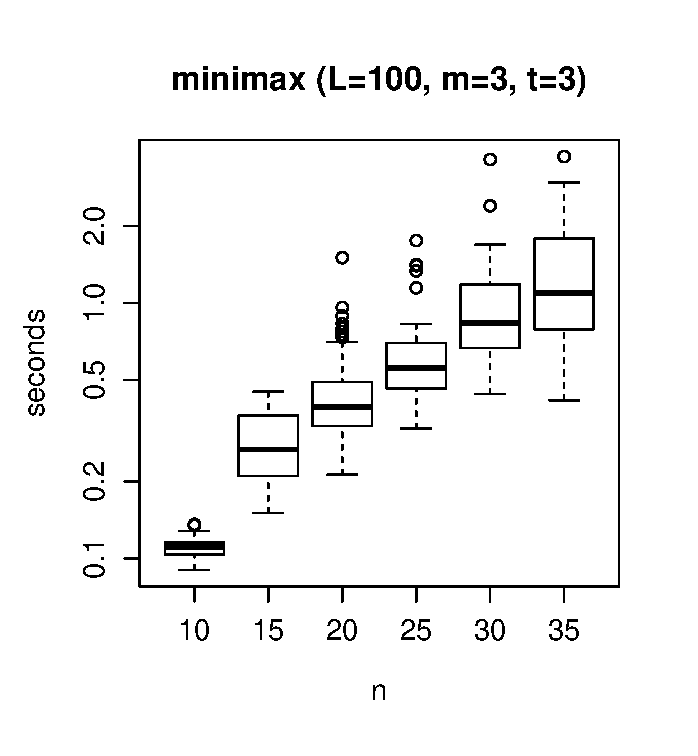
\includegraphics[width=.23\linewidth]{multi/minimax_n}
	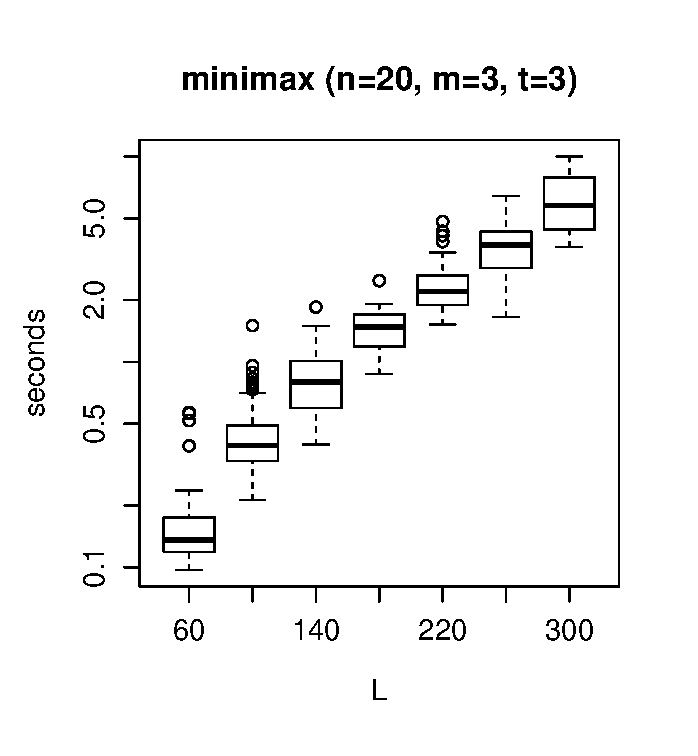
\includegraphics[width=.23\linewidth]{multi/minimax_L}
	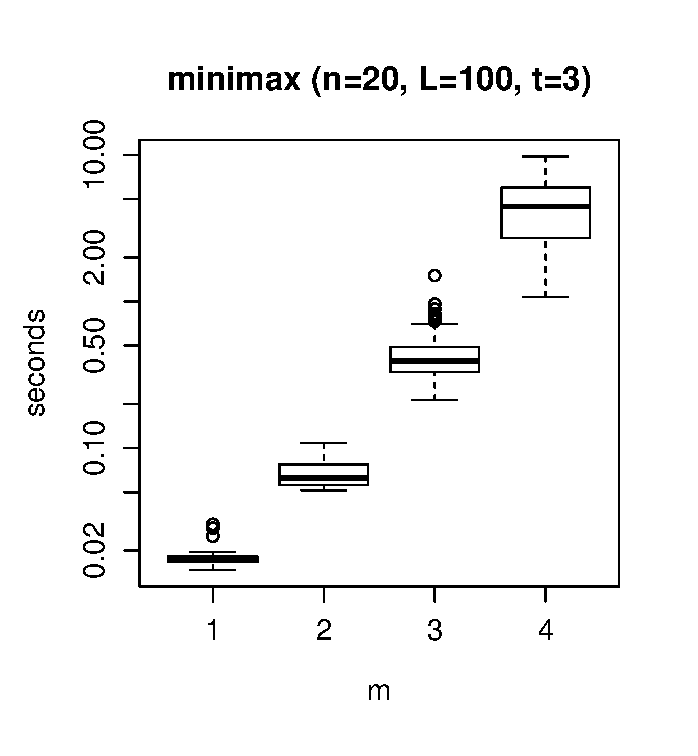
\includegraphics[width=.23\linewidth]{multi/minimax_m}
	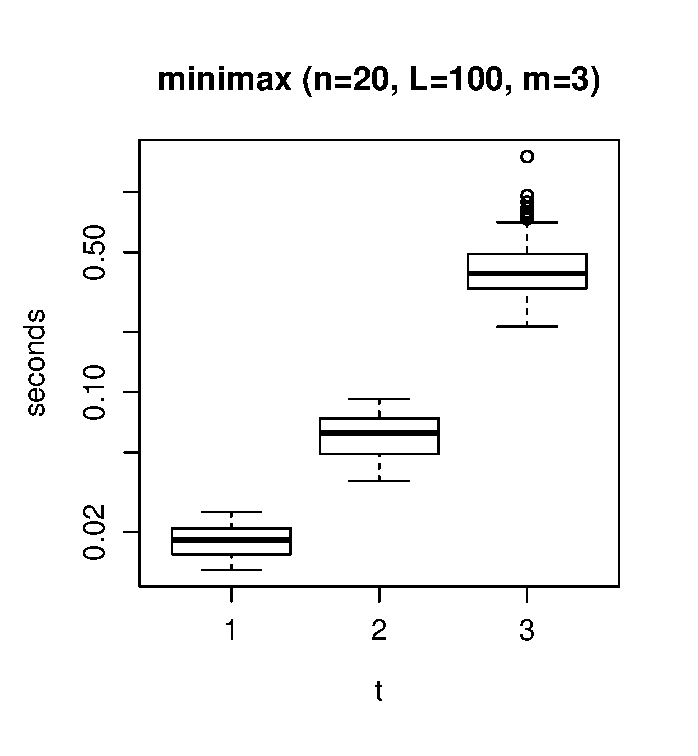
\includegraphics[width=.23\linewidth]{multi/minimax_t}\\
\vspace{-.2in}
	\caption{Running time for solving for an optimal tester strategy in
	multi-question tests.  For brevity, the parameter $m_{\text{max}}$ is denoted as $m$
	 in the title of each graph.}
	\label{fig:multi}
\end{figure*}

Figure~\ref{fig:multi} shows that DOBSS scales quite poorly 
%(exponentially)
 in
all parameters, especially in $m_{\text{max}}$ and $t$. 
As might be expected when solving MIPs, the runtime varies dramatically even for
instances of the same size, as indicated by the many outliers in the plots.
%Since solving an integer
%program involves heuristic branch-and-bound search, its running time differs a
%lot even if the sizes of MIP are the same.  Hence there are a lot of outliers
%in the box plot. 
Our general LP~(\ref{eqn:maximin}), on the other hand, scales much better
in $n, L$.  It does still struggle when scaling $m_{\text{max}}$ and $t$
(though it outperforms DOBSS).  This is expected because the size of the LP
grows exponentially in those parameters.

\subsection{Tester Utility}

One may wonder whether computing a game-theoretically optimal strategy is
worth the effort; maybe a simple heuristic performs almost as well.
To assess this, we have compared our optimal test strategies to (1) the
optimal 
strategy under the assumption that test takers do not memorize anything, and (2)
choosing $t$ questions uniformly at random from all questions.
%We compare the tester's utility of our optimal test strategies with the simple test
%strategies that draw tests from all possible question subsets of size $t$
%uniform at random. 
We generated all the test game instances as before.
(1) performed exceedingly poorly, many factors worse than the optimal
strategy.
(2) performed decently and so we only present results comparing to (2).

\begin{figure*}
	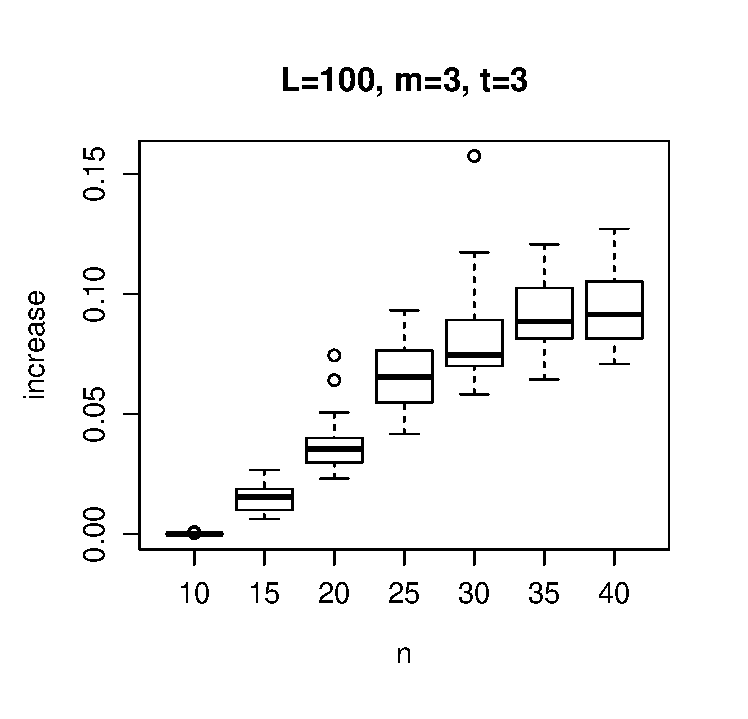
\includegraphics[width=.23\linewidth]{utility/utility_n}
	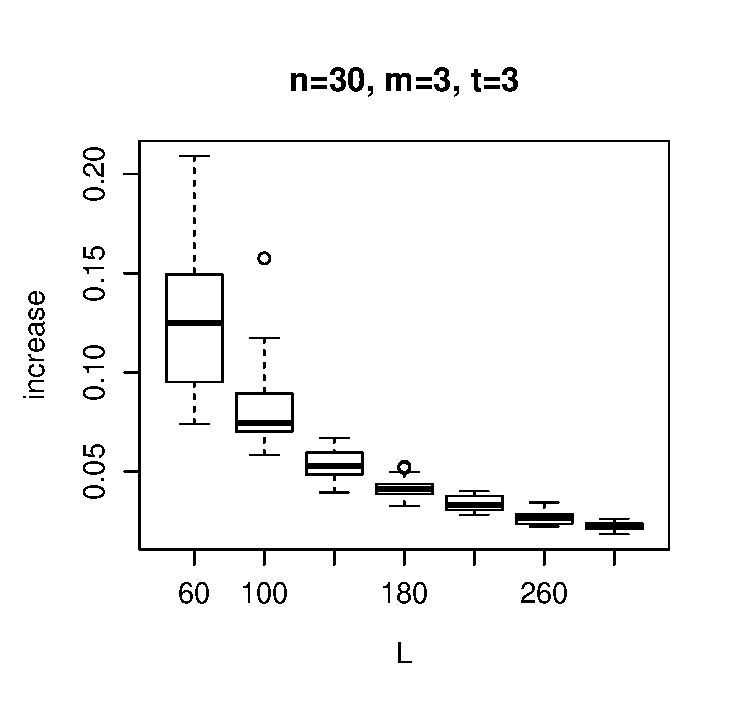
\includegraphics[width=.23\linewidth]{utility/utility_L}
	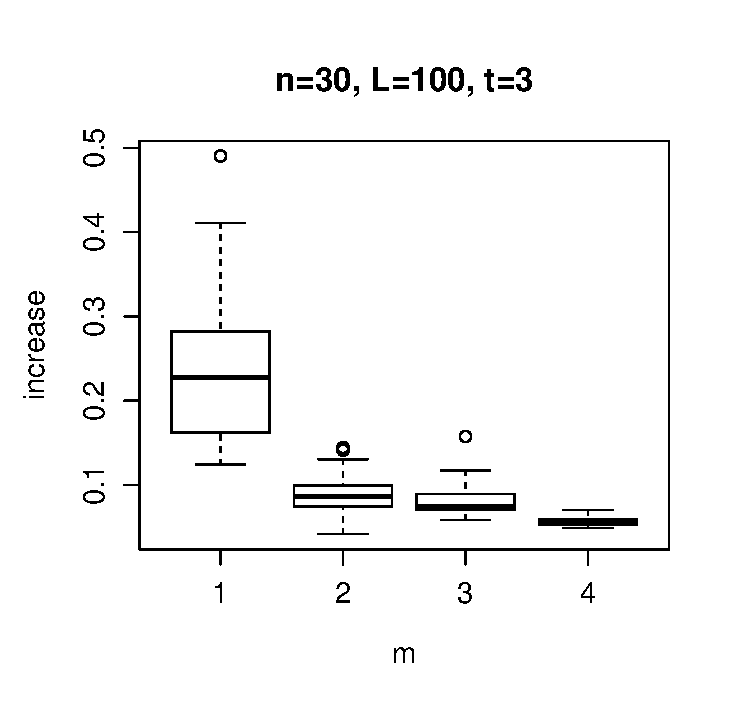
\includegraphics[width=.23\linewidth]{utility/utility_m}
	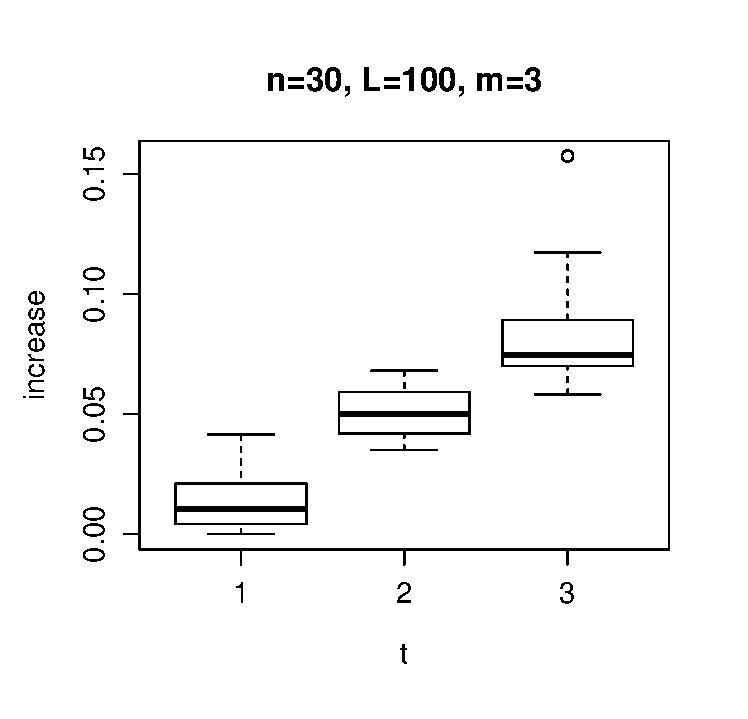
\includegraphics[width=.23\linewidth]{utility/utility_t}
	\caption{The increase in tester utility that the optimal test
          strategy gives as compared to the uniform test strategy. Letting
          the optimal utility be $u^*$ and the uniform test's utility be
          $u_0$, the number we show for the performance increase is
          $u^*/u_0-1$. For brevity, the parameter $m_{\text{max}}$ is
          denoted as $m$  in the title of each graph.}
	\label{fig:utility}
\end{figure*}

As Figure~\ref{fig:utility} indicates, the performance increase drops when
$L$ and $m$ increase, and it increases when $n$ and $t$ increase.  This is
a natural consequence of the way we generate the test game instances. The
larger $L$ and $m$ are, the more equivalent subsets of questions are likely
to be as the hardness sets start to cover the questions more uniformly; on
the other hand, the opposite is true for $n$ (for example, with large $n$,
some questions may not be hard for any type and so a waste to test) and $t$
(presumably because as $t$ grows it becomes more important to pick
questions that expose weaknesses of different types).
%Large $L$ and $m$ make each subset of questions
%more likely to be equivalent to the tester while large $n, t$ make them more
%different.

All in all, the performance of the uniform strategy is quite decent.
We suspect, though, that the way we construct the test game instances, which assumes that each
question has the same probability to be hard for a test taker, favors the
uniform strategy. In reality, we expect there to be some correlation---that
is, a question that is hard for one type is more likely to be hard for
another type as well---and presumably the uniform strategy is less
effective in this context.  Preliminary experiments on highly structured instances 
with this property confirm this intuition.
%it's more likely to have some very hard
%questions that are more likely to be hard for most test takers. Therefore
%a larger increase is expected when such factors are considered.

\section{Conclusion}

\begin{table}
%\begin{tabular}{r | c | c | c }
%	& $t = 0, 1$ & $2 \leq t \leq $const. & $t > $const.\\
%\hline
%$0 \leq m_\text{max} \leq $const. & P & P & NP-c\\
%$m_\text{max} > $const. & P & coNP-c & NP-h \& coNP-h
%\end{tabular}
\begin{tabular}{r | c | c }
	%& $0 \leq m_\text{max} \leq $ const. & $m_\text{max} > $ const. \\
	& bounded $m_\text{max}$ & unbounded $m_\text{max}$ \\
	\hline
$t=0,1$ & P & P \\
%$2 \leq t \leq$ const.
bounded $t \geq 2$ & P & coNP-c\\
%$t > $ const.
unbounded $t$ & NP-c & coNP-h and NP-h
\end{tabular}
\caption{\textsc{Optimal Test
Strategy}'s complexity ($t, m_{\max}$ are the test size and max memory size respectively)}
\label{tab:results}
\end{table}

Table~\ref{tab:results} summarizes our complexity results.
Our work is only a small first step in the design of algorithms for
game-theoretically optimal design of tests.  Future research could
focus on identifying other tractable cases.  For example, in practice,
one would expect the $H_\theta$ sets to exhibit structure that may be
exploited algorithmically.  
Another direction is to generalize beyond tests whose only outcomes
are pass and fail.
From a practical perspective, it is also
important to develop methodology to obtain the statistical information
about test taker types that is needed as input to our algorithms.
Perhaps even better than a two-phase approach, in which we first
estimate this information and then run our algorithm, would be a true
online-learning approach, where we update our testing strategy as
additional test takers take our tests.

\section*{Acknowledgments}
We thank ARO and NSF for support under grants W911NF-12-1-0550,
W911NF-11-1-0332, IIS-0953756, and CCF-1101659.


\appendix

\section{Counterexample to Zero-Sum Equivalence when the Test Taker is
  Stackelberg Leader}
\label{se:counterexample}

Let $Q=\{q_1,q_2\}$, $\Theta=\{\theta_1,\theta_2\}$,
$H_{\theta_1}=H_{\theta_2}=Q$, $m_{\theta_1}=m_{\theta_2}=1$,
$p(\theta_1)=p(\theta_2)=1/2$, $t=1$, $v_{\theta_1} = 100$, $v_{\theta_2} =
1$, $\omega_{\theta_1} = 1$, and $\omega_{\theta_2} = 100$.  If the tester
is the leader, then it is optimal for her place probability $1/2$ on each
question (and so, by Proposition~\ref{prop:equivalence}, this is also
optimal in the zero-sum version of the game).  This results in an expected
utility of $0.5$ for a test taker of type $\theta_1$, and one of $50$ for a
test taker of type $\theta_2$---so an expected utility of $25.25$ for the
test taker {\em ex ante}.

However, if the test taker can commit to a strategy in the Bayesian game
{\em ex ante} (before learning his type), then he can commit to
memorize conditionally on the type as follows: $M_{\theta_1} =\{q_1\}$ and 
$M_{\theta_2} =\{q_2\}$.  Because the tester cares more about failing
$\theta_1$, she will test $q_2$.  This results in an {\em ex ante} expected
utility of $(1/2) \cdot 100 = 50$ for the test taker, which is more than
the $25.25$ from the strategy in the regular version.













%\section{Dual of the linear program and interpretation}


%% The file named.bst is a bibliography style file for BibTeX 0.99c
\bibliographystyle{named}
\bibliography{references.bib}

\end{document}

